
\documentclass{article} % For LaTeX2e
\usepackage{iclr2027_conference,times}

% Optional math commands from https://github.com/goodfeli/dlbook_notation.
%%%%% NEW MATH DEFINITIONS %%%%%

\usepackage{amsmath,amsfonts,bm}

% Mark sections of captions for referring to divisions of figures
\newcommand{\figleft}{{\em (Left)}}
\newcommand{\figcenter}{{\em (Center)}}
\newcommand{\figright}{{\em (Right)}}
\newcommand{\figtop}{{\em (Top)}}
\newcommand{\figbottom}{{\em (Bottom)}}
\newcommand{\captiona}{{\em (a)}}
\newcommand{\captionb}{{\em (b)}}
\newcommand{\captionc}{{\em (c)}}
\newcommand{\captiond}{{\em (d)}}

% Highlight a newly defined term
\newcommand{\newterm}[1]{{\bf #1}}


% Figure reference, lower-case.
\def\figref#1{figure~\ref{#1}}
% Figure reference, capital. For start of sentence
\def\Figref#1{Figure~\ref{#1}}
\def\twofigref#1#2{figures \ref{#1} and \ref{#2}}
\def\quadfigref#1#2#3#4{figures \ref{#1}, \ref{#2}, \ref{#3} and \ref{#4}}
% Section reference, lower-case.
\def\secref#1{section~\ref{#1}}
% Section reference, capital.
\def\Secref#1{Section~\ref{#1}}
% Reference to two sections.
\def\twosecrefs#1#2{sections \ref{#1} and \ref{#2}}
% Reference to three sections.
\def\secrefs#1#2#3{sections \ref{#1}, \ref{#2} and \ref{#3}}
% Reference to an equation, lower-case.
\def\eqref#1{equation~\ref{#1}}
% Reference to an equation, upper case
\def\Eqref#1{Equation~\ref{#1}}
% A raw reference to an equation---avoid using if possible
\def\plaineqref#1{\ref{#1}}
% Reference to a chapter, lower-case.
\def\chapref#1{chapter~\ref{#1}}
% Reference to an equation, upper case.
\def\Chapref#1{Chapter~\ref{#1}}
% Reference to a range of chapters
\def\rangechapref#1#2{chapters\ref{#1}--\ref{#2}}
% Reference to an algorithm, lower-case.
\def\algref#1{algorithm~\ref{#1}}
% Reference to an algorithm, upper case.
\def\Algref#1{Algorithm~\ref{#1}}
\def\twoalgref#1#2{algorithms \ref{#1} and \ref{#2}}
\def\Twoalgref#1#2{Algorithms \ref{#1} and \ref{#2}}
% Reference to a part, lower case
\def\partref#1{part~\ref{#1}}
% Reference to a part, upper case
\def\Partref#1{Part~\ref{#1}}
\def\twopartref#1#2{parts \ref{#1} and \ref{#2}}

\def\ceil#1{\lceil #1 \rceil}
\def\floor#1{\lfloor #1 \rfloor}
\def\1{\bm{1}}
\newcommand{\train}{\mathcal{D}}
\newcommand{\valid}{\mathcal{D_{\mathrm{valid}}}}
\newcommand{\test}{\mathcal{D_{\mathrm{test}}}}

\def\eps{{\epsilon}}


% Random variables
\def\reta{{\textnormal{$\eta$}}}
\def\ra{{\textnormal{a}}}
\def\rb{{\textnormal{b}}}
\def\rc{{\textnormal{c}}}
\def\rd{{\textnormal{d}}}
\def\re{{\textnormal{e}}}
\def\rf{{\textnormal{f}}}
\def\rg{{\textnormal{g}}}
\def\rh{{\textnormal{h}}}
\def\ri{{\textnormal{i}}}
\def\rj{{\textnormal{j}}}
\def\rk{{\textnormal{k}}}
\def\rl{{\textnormal{l}}}
% rm is already a command, just don't name any random variables m
\def\rn{{\textnormal{n}}}
\def\ro{{\textnormal{o}}}
\def\rp{{\textnormal{p}}}
\def\rq{{\textnormal{q}}}
\def\rr{{\textnormal{r}}}
\def\rs{{\textnormal{s}}}
\def\rt{{\textnormal{t}}}
\def\ru{{\textnormal{u}}}
\def\rv{{\textnormal{v}}}
\def\rw{{\textnormal{w}}}
\def\rx{{\textnormal{x}}}
\def\ry{{\textnormal{y}}}
\def\rz{{\textnormal{z}}}

% Random vectors
\def\rvepsilon{{\mathbf{\epsilon}}}
\def\rvtheta{{\mathbf{\theta}}}
\def\rva{{\mathbf{a}}}
\def\rvb{{\mathbf{b}}}
\def\rvc{{\mathbf{c}}}
\def\rvd{{\mathbf{d}}}
\def\rve{{\mathbf{e}}}
\def\rvf{{\mathbf{f}}}
\def\rvg{{\mathbf{g}}}
\def\rvh{{\mathbf{h}}}
\def\rvu{{\mathbf{i}}}
\def\rvj{{\mathbf{j}}}
\def\rvk{{\mathbf{k}}}
\def\rvl{{\mathbf{l}}}
\def\rvm{{\mathbf{m}}}
\def\rvn{{\mathbf{n}}}
\def\rvo{{\mathbf{o}}}
\def\rvp{{\mathbf{p}}}
\def\rvq{{\mathbf{q}}}
\def\rvr{{\mathbf{r}}}
\def\rvs{{\mathbf{s}}}
\def\rvt{{\mathbf{t}}}
\def\rvu{{\mathbf{u}}}
\def\rvv{{\mathbf{v}}}
\def\rvw{{\mathbf{w}}}
\def\rvx{{\mathbf{x}}}
\def\rvy{{\mathbf{y}}}
\def\rvz{{\mathbf{z}}}

% Elements of random vectors
\def\erva{{\textnormal{a}}}
\def\ervb{{\textnormal{b}}}
\def\ervc{{\textnormal{c}}}
\def\ervd{{\textnormal{d}}}
\def\erve{{\textnormal{e}}}
\def\ervf{{\textnormal{f}}}
\def\ervg{{\textnormal{g}}}
\def\ervh{{\textnormal{h}}}
\def\ervi{{\textnormal{i}}}
\def\ervj{{\textnormal{j}}}
\def\ervk{{\textnormal{k}}}
\def\ervl{{\textnormal{l}}}
\def\ervm{{\textnormal{m}}}
\def\ervn{{\textnormal{n}}}
\def\ervo{{\textnormal{o}}}
\def\ervp{{\textnormal{p}}}
\def\ervq{{\textnormal{q}}}
\def\ervr{{\textnormal{r}}}
\def\ervs{{\textnormal{s}}}
\def\ervt{{\textnormal{t}}}
\def\ervu{{\textnormal{u}}}
\def\ervv{{\textnormal{v}}}
\def\ervw{{\textnormal{w}}}
\def\ervx{{\textnormal{x}}}
\def\ervy{{\textnormal{y}}}
\def\ervz{{\textnormal{z}}}

% Random matrices
\def\rmA{{\mathbf{A}}}
\def\rmB{{\mathbf{B}}}
\def\rmC{{\mathbf{C}}}
\def\rmD{{\mathbf{D}}}
\def\rmE{{\mathbf{E}}}
\def\rmF{{\mathbf{F}}}
\def\rmG{{\mathbf{G}}}
\def\rmH{{\mathbf{H}}}
\def\rmI{{\mathbf{I}}}
\def\rmJ{{\mathbf{J}}}
\def\rmK{{\mathbf{K}}}
\def\rmL{{\mathbf{L}}}
\def\rmM{{\mathbf{M}}}
\def\rmN{{\mathbf{N}}}
\def\rmO{{\mathbf{O}}}
\def\rmP{{\mathbf{P}}}
\def\rmQ{{\mathbf{Q}}}
\def\rmR{{\mathbf{R}}}
\def\rmS{{\mathbf{S}}}
\def\rmT{{\mathbf{T}}}
\def\rmU{{\mathbf{U}}}
\def\rmV{{\mathbf{V}}}
\def\rmW{{\mathbf{W}}}
\def\rmX{{\mathbf{X}}}
\def\rmY{{\mathbf{Y}}}
\def\rmZ{{\mathbf{Z}}}

% Elements of random matrices
\def\ermA{{\textnormal{A}}}
\def\ermB{{\textnormal{B}}}
\def\ermC{{\textnormal{C}}}
\def\ermD{{\textnormal{D}}}
\def\ermE{{\textnormal{E}}}
\def\ermF{{\textnormal{F}}}
\def\ermG{{\textnormal{G}}}
\def\ermH{{\textnormal{H}}}
\def\ermI{{\textnormal{I}}}
\def\ermJ{{\textnormal{J}}}
\def\ermK{{\textnormal{K}}}
\def\ermL{{\textnormal{L}}}
\def\ermM{{\textnormal{M}}}
\def\ermN{{\textnormal{N}}}
\def\ermO{{\textnormal{O}}}
\def\ermP{{\textnormal{P}}}
\def\ermQ{{\textnormal{Q}}}
\def\ermR{{\textnormal{R}}}
\def\ermS{{\textnormal{S}}}
\def\ermT{{\textnormal{T}}}
\def\ermU{{\textnormal{U}}}
\def\ermV{{\textnormal{V}}}
\def\ermW{{\textnormal{W}}}
\def\ermX{{\textnormal{X}}}
\def\ermY{{\textnormal{Y}}}
\def\ermZ{{\textnormal{Z}}}

% Vectors
\def\vzero{{\bm{0}}}
\def\vone{{\bm{1}}}
\def\vmu{{\bm{\mu}}}
\def\vtheta{{\bm{\theta}}}
\def\va{{\bm{a}}}
\def\vb{{\bm{b}}}
\def\vc{{\bm{c}}}
\def\vd{{\bm{d}}}
\def\ve{{\bm{e}}}
\def\vf{{\bm{f}}}
\def\vg{{\bm{g}}}
\def\vh{{\bm{h}}}
\def\vi{{\bm{i}}}
\def\vj{{\bm{j}}}
\def\vk{{\bm{k}}}
\def\vl{{\bm{l}}}
\def\vm{{\bm{m}}}
\def\vn{{\bm{n}}}
\def\vo{{\bm{o}}}
\def\vp{{\bm{p}}}
\def\vq{{\bm{q}}}
\def\vr{{\bm{r}}}
\def\vs{{\bm{s}}}
\def\vt{{\bm{t}}}
\def\vu{{\bm{u}}}
\def\vv{{\bm{v}}}
\def\vw{{\bm{w}}}
\def\vx{{\bm{x}}}
\def\vy{{\bm{y}}}
\def\vz{{\bm{z}}}

% Elements of vectors
\def\evalpha{{\alpha}}
\def\evbeta{{\beta}}
\def\evepsilon{{\epsilon}}
\def\evlambda{{\lambda}}
\def\evomega{{\omega}}
\def\evmu{{\mu}}
\def\evpsi{{\psi}}
\def\evsigma{{\sigma}}
\def\evtheta{{\theta}}
\def\eva{{a}}
\def\evb{{b}}
\def\evc{{c}}
\def\evd{{d}}
\def\eve{{e}}
\def\evf{{f}}
\def\evg{{g}}
\def\evh{{h}}
\def\evi{{i}}
\def\evj{{j}}
\def\evk{{k}}
\def\evl{{l}}
\def\evm{{m}}
\def\evn{{n}}
\def\evo{{o}}
\def\evp{{p}}
\def\evq{{q}}
\def\evr{{r}}
\def\evs{{s}}
\def\evt{{t}}
\def\evu{{u}}
\def\evv{{v}}
\def\evw{{w}}
\def\evx{{x}}
\def\evy{{y}}
\def\evz{{z}}

% Matrix
\def\mA{{\bm{A}}}
\def\mB{{\bm{B}}}
\def\mC{{\bm{C}}}
\def\mD{{\bm{D}}}
\def\mE{{\bm{E}}}
\def\mF{{\bm{F}}}
\def\mG{{\bm{G}}}
\def\mH{{\bm{H}}}
\def\mI{{\bm{I}}}
\def\mJ{{\bm{J}}}
\def\mK{{\bm{K}}}
\def\mL{{\bm{L}}}
\def\mM{{\bm{M}}}
\def\mN{{\bm{N}}}
\def\mO{{\bm{O}}}
\def\mP{{\bm{P}}}
\def\mQ{{\bm{Q}}}
\def\mR{{\bm{R}}}
\def\mS{{\bm{S}}}
\def\mT{{\bm{T}}}
\def\mU{{\bm{U}}}
\def\mV{{\bm{V}}}
\def\mW{{\bm{W}}}
\def\mX{{\bm{X}}}
\def\mY{{\bm{Y}}}
\def\mZ{{\bm{Z}}}
\def\mBeta{{\bm{\beta}}}
\def\mPhi{{\bm{\Phi}}}
\def\mLambda{{\bm{\Lambda}}}
\def\mSigma{{\bm{\Sigma}}}

% Tensor
\DeclareMathAlphabet{\mathsfit}{\encodingdefault}{\sfdefault}{m}{sl}
\SetMathAlphabet{\mathsfit}{bold}{\encodingdefault}{\sfdefault}{bx}{n}
\newcommand{\tens}[1]{\bm{\mathsfit{#1}}}
\def\tA{{\tens{A}}}
\def\tB{{\tens{B}}}
\def\tC{{\tens{C}}}
\def\tD{{\tens{D}}}
\def\tE{{\tens{E}}}
\def\tF{{\tens{F}}}
\def\tG{{\tens{G}}}
\def\tH{{\tens{H}}}
\def\tI{{\tens{I}}}
\def\tJ{{\tens{J}}}
\def\tK{{\tens{K}}}
\def\tL{{\tens{L}}}
\def\tM{{\tens{M}}}
\def\tN{{\tens{N}}}
\def\tO{{\tens{O}}}
\def\tP{{\tens{P}}}
\def\tQ{{\tens{Q}}}
\def\tR{{\tens{R}}}
\def\tS{{\tens{S}}}
\def\tT{{\tens{T}}}
\def\tU{{\tens{U}}}
\def\tV{{\tens{V}}}
\def\tW{{\tens{W}}}
\def\tX{{\tens{X}}}
\def\tY{{\tens{Y}}}
\def\tZ{{\tens{Z}}}


% Graph
\def\gA{{\mathcal{A}}}
\def\gB{{\mathcal{B}}}
\def\gC{{\mathcal{C}}}
\def\gD{{\mathcal{D}}}
\def\gE{{\mathcal{E}}}
\def\gF{{\mathcal{F}}}
\def\gG{{\mathcal{G}}}
\def\gH{{\mathcal{H}}}
\def\gI{{\mathcal{I}}}
\def\gJ{{\mathcal{J}}}
\def\gK{{\mathcal{K}}}
\def\gL{{\mathcal{L}}}
\def\gM{{\mathcal{M}}}
\def\gN{{\mathcal{N}}}
\def\gO{{\mathcal{O}}}
\def\gP{{\mathcal{P}}}
\def\gQ{{\mathcal{Q}}}
\def\gR{{\mathcal{R}}}
\def\gS{{\mathcal{S}}}
\def\gT{{\mathcal{T}}}
\def\gU{{\mathcal{U}}}
\def\gV{{\mathcal{V}}}
\def\gW{{\mathcal{W}}}
\def\gX{{\mathcal{X}}}
\def\gY{{\mathcal{Y}}}
\def\gZ{{\mathcal{Z}}}

% Sets
\def\sA{{\mathbb{A}}}
\def\sB{{\mathbb{B}}}
\def\sC{{\mathbb{C}}}
\def\sD{{\mathbb{D}}}
% Don't use a set called E, because this would be the same as our symbol
% for expectation.
\def\sF{{\mathbb{F}}}
\def\sG{{\mathbb{G}}}
\def\sH{{\mathbb{H}}}
\def\sI{{\mathbb{I}}}
\def\sJ{{\mathbb{J}}}
\def\sK{{\mathbb{K}}}
\def\sL{{\mathbb{L}}}
\def\sM{{\mathbb{M}}}
\def\sN{{\mathbb{N}}}
\def\sO{{\mathbb{O}}}
\def\sP{{\mathbb{P}}}
\def\sQ{{\mathbb{Q}}}
\def\sR{{\mathbb{R}}}
\def\sS{{\mathbb{S}}}
\def\sT{{\mathbb{T}}}
\def\sU{{\mathbb{U}}}
\def\sV{{\mathbb{V}}}
\def\sW{{\mathbb{W}}}
\def\sX{{\mathbb{X}}}
\def\sY{{\mathbb{Y}}}
\def\sZ{{\mathbb{Z}}}

% Entries of a matrix
\def\emLambda{{\Lambda}}
\def\emA{{A}}
\def\emB{{B}}
\def\emC{{C}}
\def\emD{{D}}
\def\emE{{E}}
\def\emF{{F}}
\def\emG{{G}}
\def\emH{{H}}
\def\emI{{I}}
\def\emJ{{J}}
\def\emK{{K}}
\def\emL{{L}}
\def\emM{{M}}
\def\emN{{N}}
\def\emO{{O}}
\def\emP{{P}}
\def\emQ{{Q}}
\def\emR{{R}}
\def\emS{{S}}
\def\emT{{T}}
\def\emU{{U}}
\def\emV{{V}}
\def\emW{{W}}
\def\emX{{X}}
\def\emY{{Y}}
\def\emZ{{Z}}
\def\emSigma{{\Sigma}}

% entries of a tensor
% Same font as tensor, without \bm wrapper
\newcommand{\etens}[1]{\mathsfit{#1}}
\def\etLambda{{\etens{\Lambda}}}
\def\etA{{\etens{A}}}
\def\etB{{\etens{B}}}
\def\etC{{\etens{C}}}
\def\etD{{\etens{D}}}
\def\etE{{\etens{E}}}
\def\etF{{\etens{F}}}
\def\etG{{\etens{G}}}
\def\etH{{\etens{H}}}
\def\etI{{\etens{I}}}
\def\etJ{{\etens{J}}}
\def\etK{{\etens{K}}}
\def\etL{{\etens{L}}}
\def\etM{{\etens{M}}}
\def\etN{{\etens{N}}}
\def\etO{{\etens{O}}}
\def\etP{{\etens{P}}}
\def\etQ{{\etens{Q}}}
\def\etR{{\etens{R}}}
\def\etS{{\etens{S}}}
\def\etT{{\etens{T}}}
\def\etU{{\etens{U}}}
\def\etV{{\etens{V}}}
\def\etW{{\etens{W}}}
\def\etX{{\etens{X}}}
\def\etY{{\etens{Y}}}
\def\etZ{{\etens{Z}}}

% The true underlying data generating distribution
\newcommand{\pdata}{p_{\rm{data}}}
% The empirical distribution defined by the training set
\newcommand{\ptrain}{\hat{p}_{\rm{data}}}
\newcommand{\Ptrain}{\hat{P}_{\rm{data}}}
% The model distribution
\newcommand{\pmodel}{p_{\rm{model}}}
\newcommand{\Pmodel}{P_{\rm{model}}}
\newcommand{\ptildemodel}{\tilde{p}_{\rm{model}}}
% Stochastic autoencoder distributions
\newcommand{\pencode}{p_{\rm{encoder}}}
\newcommand{\pdecode}{p_{\rm{decoder}}}
\newcommand{\precons}{p_{\rm{reconstruct}}}

\newcommand{\laplace}{\mathrm{Laplace}} % Laplace distribution

\newcommand{\E}{\mathbb{E}}
\newcommand{\Ls}{\mathcal{L}}
\newcommand{\R}{\mathbb{R}}
\newcommand{\emp}{\tilde{p}}
\newcommand{\lr}{\alpha}
\newcommand{\reg}{\lambda}
\newcommand{\rect}{\mathrm{rectifier}}
\newcommand{\softmax}{\mathrm{softmax}}
\newcommand{\sigmoid}{\sigma}
\newcommand{\softplus}{\zeta}
\newcommand{\KL}{D_{\mathrm{KL}}}
\newcommand{\Var}{\mathrm{Var}}
\newcommand{\standarderror}{\mathrm{SE}}
\newcommand{\Cov}{\mathrm{Cov}}
% Wolfram Mathworld says $L^2$ is for function spaces and $\ell^2$ is for vectors
% But then they seem to use $L^2$ for vectors throughout the site, and so does
% wikipedia.
\newcommand{\normlzero}{L^0}
\newcommand{\normlone}{L^1}
\newcommand{\normltwo}{L^2}
\newcommand{\normlp}{L^p}
\newcommand{\normmax}{L^\infty}

\newcommand{\parents}{Pa} % See usage in notation.tex. Chosen to match Daphne's book.

\DeclareMathOperator*{\argmax}{arg\,max}
\DeclareMathOperator*{\argmin}{arg\,min}

\DeclareMathOperator{\sign}{sign}
\DeclareMathOperator{\Tr}{Tr}
\let\ab\allowbreak


\usepackage{hyperref}
\usepackage{url}



\usepackage{amsmath,amssymb,booktabs,graphicx,microtype,xcolor,enumitem,multirow}
\usepackage{flafter}
% \usepackage{tikz}
% \usetikzlibrary{arrows.meta,positioning,fit}
\usepackage{hyperref,url}
\definecolor{dynblue}{HTML}{DCEBFA}
\definecolor{physorange}{HTML}{FBE4CB}
\definecolor{datagreen}{HTML}{DDEFD8}
\definecolor{learnpurple}{HTML}{E9DDF2}
\definecolor{projred}{HTML}{F5D4D4}
\newcommand{\done}{\(\boxtimes\)}
\newcommand{\todo}{\(\square\)}
\newcommand{\model}{\textsc{DiffMars}}
% \newcommand{\Ls}{L_\mathrm{s}}
\newcommand{\fast}{\textit{Fast strategy:}}
\newcommand{\evidence}{\textit{Evidence:}}
\newcommand{\pending}[1]{\textcolor{blue!65!black}{[To complete: #1]}}


\graphicspath{{assets/}{./}}
\newcommand{\co}{CO$_2$}


\title{AEGIS: Differentiable Mars Climate Model with Neural Closures}

% Authors must not appear in the submitted version. They should be hidden
% as long as the \iclrfinalcopy macro remains commented out below.
% Non-anonymous submissions will be rejected without review.

\iclrfinalcopy

\author{Sameera S Kashyap, Victor Cruz, Angel Yepez  \& Razvan Marinescu \\
Department of Computer Science\\
UC Santa Cruz\\
Santa Cruz, CA 95064, USA \\
\texttt{\{ssudars1, vcruz17, ayepezal, ramarine\}@ucsc.edu} \\
% \And
% Ji Q. Ren \& Yevgeny LeNet \\
% Department of Computational Neuroscience \\
% University of the Witwatersrand \\
% Joburg, South Africa \\
% \texttt{\{robot,net\}@wits.ac.za} \\
% \AND
% Coauthor \\
% Affiliation \\
% Address \\
% \texttt{email}
}

% The \author macro works with any number of authors. There are two commands
% used to separate the names and addresses of multiple authors: \And and \AND.
%
% Using \And between authors leaves it to \LaTeX{} to determine where to break
% the lines. Using \AND forces a linebreak at that point. So, if \LaTeX{}
% puts 3 of 4 authors names on the first line, and the last on the second
% line, try using \AND instead of \And before the third author name.

\newcommand{\fix}{\marginpar{FIX}}
\newcommand{\new}{\marginpar{NEW}}

\begin{document}
\maketitle
\begin{abstract}                                                      
General circulation models (GCMs) are the primary tool for simulating planetary atmospheres. They play a vital role in understanding Mars's atmosphere, as forecasting its unique weather is mission-critical for operations such as entry, descent, and landing. Mars poses unusual challenges for these models, as observations are sparse compared to Earth.  In addition, a thin \co{} atmosphere alongside a radiatively active dust cycle creates a volatile atmosphere with large diurnal temperature swings and no true terrestrial analog for validation. Existing Mars GCMs, including the LMD PCM, the NASA Ames Mars GCM, and PlanetWRF, are mature and physically detailed but are implemented in legacy Fortran with finite-difference or finite-volume solvers, and they do not expose gradients for calibration or machine learning. Here we present AEGIS, a modular differentiable Mars climate model that couples Mars's unique atmospheric physics to the Dinosaur dynamical core, with interfaces for neural closures. We demonstrate coupled forward integration, physical-parameter derivatives, and neural training. Historical seasonal comparisons show terrain-correlated surface pressure but also warm temperature biases and substantial frost and wind errors. The atmosphere--frost inventory is constrained by a numerical projection; its small residual does not establish raw energy or momentum conservation. We separate historical results from a new fixed-update neural-radiation comparison and state the remaining long-run, calibration, and observational validation requirements.
\end{abstract}

\section{Introduction}
General circulation models (GCMs) connect the governing equations of atmospheric motion to the physical processes that shape planetary climate. Established Mars models include the LMD Mars GCM, the NASA Ames Mars GCM, and PlanetWRF \citep{forget1999,haberle1993,richardson2007}. On Mars, radiative heating by dust and \co{}, exchange with a thermally active surface, and seasonal condensation onto polar caps jointly shape circulation, pressure, and frost. A useful model must represent these interactions while allowing individual assumptions to be tested \citep{forget2010co2cycle}.

Traditional GCMs contain uncertain parameterization coefficients whose
coupled effects can complicate tuning and permit compensating errors
\citep{forget1999}. Parameter sweeps and ensemble calibration are often computationally expensive \citep{cleary2020augmented}. In addition, the forward-model interface does not generally expose gradients, and maintaining separate adjoint implementations incurs substantial development effort \citep{giering1998}. Introducing a learned component can also require substantial changes to the coupling between numerical and physical routines. These challenges motivate models in which physical simulation and gradient optimization share the same implementation \citep{davenport2026}.

Differentiable programming bridges this gap. When a simulation is
implemented as differentiable numerical operations, automatic differentiation applies the chain rule through its computational graph to obtain derivatives of outputs with respect to inputs and parameters or learned weights \citep{baydin2018autodiff}. This supports calibration, sensitivity analysis, inverse problems, and training over multiple time steps. In particular, a neural parameterization can be optimized for its effect on a coupled trajectory, accounting for feedback between the learned tendency and the resolved dynamics \citep{rasp2020, kashyap2024modelingchaoticlorenzode}. NeuralGCM demonstrates the potential of this approach for Earth's weather and climate by coupling learned parameterizations to a differentiable atmospheric dynamical core \citep{kochkov2024}. Its Dinosaur core solves the hydrostatic primitive equations using spectral horizontal coordinates and a sigma vertical coordinate. The JAX Circulation Model (JCM) uses the same core with an explicit suite of intermediate-complexity physical parameterizations, providing a setting for process-based studies and hybrid modeling for Earth's climate and atmosphere \citep{gelbrecht2023differentiable, davenport2026}. In a different physical domain, JAX MD illustrates how reusable numerical components and neural models can be composed within a common differentiable simulation environment \citep{schoenholz2020}. AEGIS shares the Dinosaur backbone with JCM and NeuralGCM, but addresses a different physical regime and adds coupled state variables and operators needed for Mars.

% Applying this approach to Mars requires more than substituting planetary
% constants into an Earth configuration. Mars has a thin,
% CO$_2$-dominated atmosphere, radiatively active dust, large terrain
% variations, and strong surface thermal forcing that comprises a substantial fraction of atmospheric mass. Its seasonal CO$_2$ frost cycle changes surface pressure and the surface energy budget \citep{haberle2019ames,piqueux2024co2seasonal}. These processes require planetary radiation, surface, and mass-exchange operators. AEGIS supplies these components and extends the state and time-step coupling around Dinosaur to carry the surface reservoirs and evolving atmospheric inventory.

In this work, we present AEGIS, a differentiable Mars Climate Model based on the Dinosaur Core. Unlike the Earth-focused configurations of its Dinosaur-based predecessors, AEGIS uses planetary radius, rotation, and thermodynamic scales at the dynamical interface. It adds Mars radiation and surface physics, evolves frost and regolith alongside the atmosphere, feeds \co{} phase change into the dynamical core's prognostic log-pressure state, and projects the coupled atmosphere--frost inventory after each step. These additions make mass exchange and surface memory part of the differentiated trajectory.

We make three contributions:
\begin{enumerate}[leftmargin=*,nosep]
\item We extend the Dinosaur core with planetary-unit rescaling, a coupled atmosphere--surface--frost--regolith state, \co{} mass exchange into prognostic pressure, and an atmosphere--frost inventory projection.
\item We provide modular Mars radiation, surface, transport, and neural interfaces through which physical controls and learned components can enter the same coupled simulation.
\item We verify physical and neural gradients, evaluate Mars fields against reference products, and demonstrate calibration, year-long forward integration, and controlled neural experiments, and showcase them in Section~\ref{sec:results}.
\end{enumerate}

\section{Methods}
AEGIS couples a modular Mars physics suite to the Dinosaur spectral dynamical core, carrying the atmosphere, surface, \co{} frost, and regolith in a single differentiable state (Section~\ref{sec:framework}). Automatic differentiation through this coupled time step provides gradients for physical calibration and for training learned components that enter through a common neural interface (Section~\ref{sec:differentiation}).

 \subsection{Atmospheric configurations and the dynamical framework}\label{sec:framework}

AEGIS separates the description of a planetary atmosphere from the numerical machinery used to evolve it. A body configuration specifies radius $a$, gravity $g$, rotation rate $\Omega$, specific gas constant $R$, heat capacity $c_p$, and reference temperature and pressure. We use Mars values for the planetary constants \citep{nasaMarsFactSheet}. The dynamical equations consume these values through a common interface. Length and time are scaled by $a$ and $(2\Omega)^{-1}$, respectively, so the nondimensional radius and rotation rate follow Dinosaur's conventions for each body, removing dependence on Earth-specific default scales while retaining the existing spectral operators.

The framework supports a hierarchy of atmospheric configurations. Dynamical configurations isolate resolved transport; physically forced configurations add radiation, surface exchange, mixing, and volatile reservoirs; hybrid configurations add a learned tendency or substitute a learned component at a selected physical interface. Complexity is therefore introduced through explicit components: a body definition establishes the mechanical and thermodynamic constants, while its radiation, condensables, and boundary conditions establish the atmospheric regime. The physically developed configuration evaluated here is Mars; extending to another atmosphere involves supplying the relevant process operators as well as its constants \citep{hu2025stablemachinelearningparameterizationsubgrid}.

Dinosaur advances the hydrostatic primitive equations on a sphere \citep{kochkov2024,davenport2026}. The atmospheric state contains spectral vorticity and divergence, temperature relative to a reference profile, log surface pressure, optional transported tracers, and simulation time, on a vertical coordinate $\sigma=p/p_s$ that follows changes in atmospheric mass and the terrain-dependent lower boundary \citep{kochkov2024}. 
Spectral transform models using sigma coordinates have a long history in Mars atmospheric modeling \citep{wilson1997stationarywaves}. The main experiments use triangular truncation T21, a $64\times32$ longitude--latitude transform grid, and 12 equally spaced sigma layers.

The coupled state augments the atmospheric variables with surface temperature, pressure-equivalent \co{} frost, and a vertical regolith temperature profile attached to their geographic columns. Writing the full state as $\vx$, the coupled equations take the form
\begin{equation}
 \frac{d\vx}{dt}=\mathcal{D}_{\mathrm{imp}}(\vx)
 +\mathcal{D}_{\mathrm{exp}}(\vx)
 +\mathcal{P}_{\boldsymbol{\alpha}}(\vx,t)
 +\mathcal{N}_{\boldsymbol{\theta}}(\vx,t),
 \label{eq:coupled}
\end{equation}
where $\mathcal{D}$ denotes resolved dynamics, $\mathcal{P}_{\boldsymbol{\alpha}}$ denotes physical parameterizations with parameters $\boldsymbol{\alpha}$, and $\mathcal{N}_{\boldsymbol{\theta}}$ denotes an optional neural tendency. A neural replacement for a physical component is composed inside $\mathcal{P}$ instead of being added a second time. Time integration uses Dinosaur's implicit--explicit SIL3 Runge--Kutta scheme \citep{whitaker2013}, with linear gravity-wave terms treated implicitly and nonlinear dynamics and assembled physical tendencies on the explicit side. Planetary unit conversion, the augmented state, and the atmosphere--frost correction are implemented in AEGIS's surrounding operators.

\begin{figure}[t]
\centering
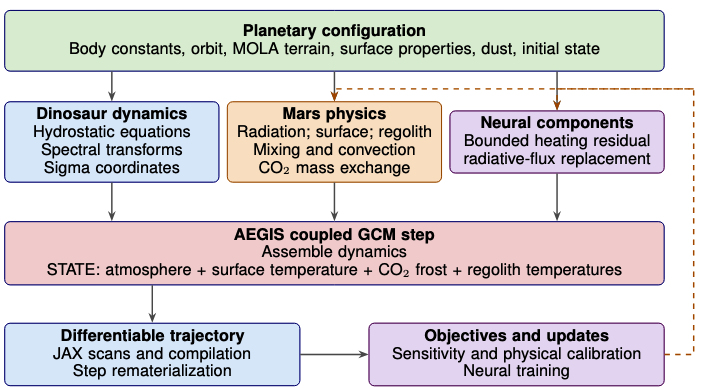
\includegraphics[width=.65\linewidth]{assets/architecture.png}
\caption{AEGIS architecture. Planetary constants and boundary data configure a shared GCM. Dinosaur supplies resolved dynamics; Mars physical operators supply column tendencies and surface evolution; neural components enter as bounded residuals or component replacements. The coupled time step advances atmosphere and surface reservoirs. Trajectory objectives connect the simulated fields to physical-parameter calibration and neural training through automatic differentiation. Dashed arrows denote this gradient-based update path.}
\label{fig:architecture}
\end{figure}

The Mars operators in $\mathcal{P}_{\boldsymbol{\alpha}}$ span \co{} and dust radiation, surface and regolith energy exchange, boundary-layer mixing and dry convection, and a \co{} condensation cycle \citep{lacis1991,forget1999,haberle2019ames,petrosyan2011pbl}. The last is the distinctive Mars coupling: surface condensation and sublimation transfer mass between the atmosphere and frost, feeding the prognostic log surface pressure,
\begin{equation}
 \left.\frac{d\log p_s}{dt}\right|_{\mathrm{phase}}
 =-\frac{1}{p_s}\frac{dI}{dt},
 \label{eq:mass}
\end{equation}

Here, \(p_s\) is local surface pressure and \(I=g m_{\mathrm{ice}}\) is the surface frost inventory in pressure units. Positive \(dI/dt\) denotes condensation onto the surface and lowers \(p_s\); negative \(dI/dt\) denotes sublimation and raises \(p_s\). The factor \(1/p_s\) converts the pressure tendency to a log-pressure tendency. A per-step projection constrains the integrated atmosphere-plus-frost inventory to the specified mass budget. Its residual measures satisfaction of that constraint, not unprojected discretization error or full energy/momentum closure. Because \co{} is both a radiative gas and a substantial mobile mass reservoir, carrying its phase change through the prognostic pressure state, alongside surface and subsurface temperatures \citep{kellyseaonalpolar}, makes this coupling part of the simulated system and its derivatives. The radiation, surface, boundary-layer, and \co{}-inventory operators are detailed in Appendix~\ref{app:physics}.

\subsection{Differentiation and neural components}\label{sec:differentiation}

Let \(\Phi_{\boldsymbol{\alpha},\boldsymbol{\theta}}\) denote the operator that propagates a single time step, including the reservoir corrections. A trajectory is the repeated composition of $\vx_{n+1}=\Phi_{\boldsymbol{\alpha},\boldsymbol{\theta}}(\vx_n)$ while a loss function can be evaluated over an entire trajectory rollout as $\mathcal{L}(\boldsymbol{\alpha},\boldsymbol{\theta})=\ell\bigl(\mathcal{H}(\vx_1),\vy_1,\mathcal{H}(\vx_2),\vy_2,\ldots,\mathcal{H}(\vx_N),\vy_N\bigr)$, where \(\mathcal{H}\) extracts evaluated fields and \(\vy_n\) denotes the target data at step \(n\). JAX differentiates this discrete numerical trajectory using automatic differentiation. We use forward-mode differentiation for the three physical controls and reverse-mode differentiation for neural weights; forward mode efficiently evaluates derivatives with respect to a small number of controls, whereas reverse mode is appropriate for a scalar loss with many parameters \citep{baydin2018autodiff,jax2024autodiff}. Reverse-mode training through coupled rollouts, as in the heating experiment below, uses fixed-length scans with step rematerialization, which trades additional computation for reduced reverse-mode memory use by recomputing selected forward intermediates during the backward pass \citep{jax2024checkpoint}.


Learned components are exposed through two adapters that share one interface: a model is initialized from a random key into a JAX parameter tree, input normalization is fitted on training data only, and a \texttt{bind} call returns a pure JAX function that is passed to the coupled equations when the time step is built. The residual adapter adds a bounded heating tendency computed from current-state column features: the temperature profile, surface temperature and pressure, lowest-layer winds, geographic coordinates, and insolation, 21 features at T21/L12, as the equation
\begin{equation}
 \dot T_{\mathrm{NN}}=h_{\max}\tanh f_{\boldsymbol{\theta}}(\vz),
 \label{eq:neural}
\end{equation}
where $f_{\boldsymbol{\theta}}$ is the network, $\vz$ the normalized column features, and $h_{\max}$ a fixed heating bound, converts it to the dynamical core's tendency units, and adds it to the physical tendencies while leaving the surface reservoirs under physical control; a zero-initialized output layer reproduces the physical model exactly at the start of training. The replacement adapter is a drop-in radiation component: it predicts interface fluxes from the column temperature and pressure profiles, dust, sunlight, albedo, and emissivity, bounds shortwave fluxes by the incoming sunlight, keeps longwave fluxes positive, imposes the top and surface boundary conditions exactly, and computes heating from flux convergence, so the column energy budget closes for any network weights. Both adapters accept a custom network through an \texttt{apply(params, features)} function and check the vertical grid and radiation configuration when bound. Because a bound component is part of the coupled step, its parameters can be trained on local targets or by reverse-mode differentiation through rollouts, and they are saved together with their normalization and metadata in validated checkpoints. Training protocols for the reported experiments are given in Appendix~\ref{app:protocol}.

% We demonstrate the learning abilities of AEGIS by training two neural components that refine the climate dynamics. The first neural component adds a bounded atmospheric heating tendency. It consumes the current temperature profile, surface temperature, surface pressure, lowest-layer winds, geographic coordinates, and insolation. At T21/L12 this gives 21 features per column. The model uses a shared multilayer perceptron with one eight-unit GELU hidden layer and one output, for 185 trainable parameters. Its heating is
% \begin{equation}
%  \dot T_{\mathrm{NN}}=h_{\max}\tanh f_{\theta}(z),
%  \qquad h_{\max}=2\times10^{-4}\ \mathrm{K\,s^{-1}}.
%  \label{eq:neural}
% \end{equation}
% The scalar output is broadcast across the atmospheric layers of each column and converted to the dynamical core's tendency units. The final layer is initialized to zero, giving the physical model at initialization. Because the correction enters each time step, its effect propagates through subsequent circulation and physical tendencies. A custom network can be supplied through the adapter; experiments with vertically resolved outputs or other prognostic tendencies can extend the same contract with corresponding physical constraints.

% The second neural component replaces the radiation term with predicted interface fluxes. Its inputs include atmospheric temperature and pressure profiles, surface temperature, dust properties, sunlight, albedo, and emissivity. Shortwave outputs are bounded fractions of incoming sunlight, longwave outputs are positive, and the prescribed top and surface boundary conditions are imposed explicitly. Heating is calculated from flux convergence, preserving the column energy accounting. In the experiments reported here, the learned operator emulates the compact multiband radiation scheme on generated four-layer columns with fixed pressure, dust, and illumination per column, and the trained operator is also run inside the coupled T21 model. This setting supports comparisons between local flux fitting and trajectory-based training while retaining a common coupling to the GCM. Finally, we test the same differentiable inverse workflow without a neural network by recovering a known surface-exchange multiplier in the column model. The calibration and neural-training protocols---reanalysis windows, initialization, loss weighting, optimization, and the neural-radiation setup---are detailed in Appendix~\ref{app:protocol}.


\section{Results}\label{sec:results}
% \subsection{Verified gradients through the coupled Mars model}

% \begin{table}[t]
% \centering
% \small
% \caption{Derivative checks through coupled AEGIS-Mars trajectories. All
% comparisons satisfy
% \(\lvert g_{\mathrm{AD}}-g_{\mathrm{FD}}\rvert
% \leq10^{-8}+10^{-4}\lvert g_{\mathrm{FD}}\rvert\).}
% \label{tab:derivative_checks}
% \begin{tabular}{llccc}
% \toprule
% Category & Objective & Horizon & Checks & Passed \\
% \midrule
% Physical sensitivity &
% Final mean atmospheric temperature &
% 1--148 steps &
% 54 &
% 54/54 \\

% Physical calibration &
% Scalar fitting objective &
% task-dependent &
% 9 &
% 9/9 \\

% Neural fitting &
% Multi-field trajectory objective &
% 25 steps &
% 3 &
% 3/3 \\
% \bottomrule
% \label{diff-table}
% \end{tabular}
% \end{table}


% We verify derivatives through both a scalar atmospheric diagnostic and the objectives used for physical calibration and neural fitting. The physical derivative experiment differentiates final area- and layer-mean atmospheric temperature with respect to the three physical controls. It compares automatic differentiation (AD) with centered finite differences (FD) over six rollout horizons, from 1 to 148 steps, corresponding to 300--44{,}400\,s at a 300\,s
% timestep. For each control and horizon, FD estimates use perturbations
% \(10^{-3}\), \(10^{-4}\), and \(10^{-5}\), yielding 54 comparisons through the coupled dynamics and Mars physics given by Table \ref{diff-table}. All 54 physical-sensitivity checks pass the recorded criterion. At the longest horizon, \(44{,}400\,\mathrm{s}\), the largest discrepancy is \(3.56\times10^{-7}\). Agreement across perturbation sizes and integration horizons supports the use of the computed derivatives for physical-parameter sensitivity in these coupled simulations.

% The historical twelve-window pilot reduces test temperature RMSE from 2.45505 to 2.39699\,K, a 0.05805\,K gain (Table~\ref{tab:skill}). A paired-year percentile interval conditional on the two held-out Mars years is [0.03512, 0.08693]\,K; four windows and one fitted run do not establish population skill or optimizer uncertainty. Training loss was still decreasing over the last five of the 50 Adam updates, so convergence was not established. The validation-selected physical controls were (0.902924, 1.096341, 0.816336). These historical results require regeneration after the PBL and sidereal-clock fixes; the revised runner records bounded multi-start optimizer termination and projected gradients rather than equating a fixed update budget with convergence.

% \begin{table}[t]\centering\small
\caption{Historical reference characterization, using the arithmetic mean of four seasonal statistics per row (not pooled spatial RMSE). Bias is model minus reference. Temporal sampling and wind heights are unmatched; opacity controls were Ames-informed.}
\label{tab:reference}\label{mola-table}
\begin{tabular}{llrrr}\toprule
Reference & Field & Bias & RMSE & Correlation \\\midrule
NASA Ames & Pressure (Pa) & -40.92 & 52.37 & 0.986 \\
NASA Ames & Temperature (K) & +3.46 & 20.64 & 0.789 \\
NASA Ames & Wind (m/s) & +9.75 & 11.91 & 0.442 \\
NASA Ames & Frost (Pa-eq.) & +7.31 & 168.48 & 0.816 \\
MCD 6.1 & Pressure (Pa) & -41.56 & 57.18 & 0.977 \\
MCD 6.1 & Temperature (K) & +7.12 & 21.58 & 0.787 \\
MCD 6.1 & Wind (m/s) & +6.91 & 10.03 & 0.263 \\
MCD 6.1 & Frost (Pa-eq.) & -5.69 & 196.28 & 0.806 \\
ARCO-MACDA & Pressure (Pa) & +3.43 & 40.72 & 0.988 \\
ARCO-MACDA & Temperature (K) & +7.42 & 22.27 & 0.772 \\
ARCO-MACDA & Wind (m/s) & +2.90 & 7.88 & 0.454 \\
ARCO-MACDA & Frost (Pa-eq.) & -65.55 & 368.34 & 0.795 \\
\bottomrule\end{tabular}\end{table}



\subsection{Verified gradients through the coupled Mars model}

\begin{table}[t]
\centering
\small
\caption{Derivative checks through coupled AEGIS trajectories. All
comparisons satisfy
\(\lvert g_{\mathrm{AD}}-g_{\mathrm{FD}}\rvert
\leq10^{-8}+10^{-4}\lvert g_{\mathrm{FD}}\rvert\).}
\label{tab:derivative_checks}
\begin{tabular}{llccc}
\toprule
Category & Objective & Horizon & Checks & Passed \\
\midrule
Physical sensitivity &
Final mean atmospheric temperature &
1--148 steps &
54 &
54/54 \\

Physical calibration &
Scalar fitting objective &
task-dependent &
9 &
9/9 \\

Neural fitting &
Multi-field trajectory objective &
25 steps &
3 &
3/3 \\

Multi-diagnostic sensitivity &
Mean surface $T$, $p_s$, and \co{} frost &
74--1480 steps &
9 &
9/9 \\
\bottomrule
\label{diff-table}
\end{tabular}
\end{table}


We verify derivatives through both a scalar atmospheric diagnostic and the objectives used for physical calibration and neural fitting. The physical derivative experiment differentiates final area- and layer-mean atmospheric temperature with respect to the three physical controls. It compares automatic differentiation (AD) with centered finite differences (FD) over six rollout horizons, from 1 to 148 steps, corresponding to 300--44{,}400\,s at a 300\,s
timestep. For each control and horizon, FD estimates use perturbations
\(10^{-3}\), \(10^{-4}\), and \(10^{-5}\), yielding 54 comparisons through the coupled dynamics and Mars physics given by Table \ref{diff-table}. All 54 physical-sensitivity checks pass the recorded criterion. At the longest horizon, \(44{,}400\,\mathrm{s}\), the largest discrepancy is \(3.56\times10^{-7}\). Agreement across perturbation sizes and integration horizons supports the use of the computed derivatives for physical-parameter sensitivity in these coupled simulations.

We extend this verification to multi-day rollouts and to several coupled diagnostics at once. Starting from a MY32, $L_s=45^\circ$ ARCO-MACDA window, we compute the forward-mode Jacobian \texttt{jax.jacfwd} of global-mean surface temperature, surface pressure, and surface \co{} frost with respect to the \co{} longwave opacity multiplier $\beta$ at its nominal value $\beta=1$, through the complete coupled rollout at horizons of 0.25, 1, and 5 sols (74, 296, and 1480 steps). All nine derivatives agree with centered finite differences ($\epsilon=10^{-3}$), with a maximum relative discrepancy of $3.99\times10^{-6}$ (Fig.~\ref{fig:co2-sensitivity}). The sensitivities are physically interpretable: increasing \co{} longwave opacity warms the surface, with $\partial\bar T_s/\partial\beta$ growing from 0.488 to 0.785 and 0.945\,K per unit $\beta$ as the response accumulates, and the warmer surface suppresses condensation, so surface pressure rises while frost falls ($\partial\bar p_s/\partial\beta$ grows from $2.94\times10^{-3}$ to $4.66\times10^{-2}$\,Pa). The pressure and frost derivatives are equal and opposite at every horizon, with their sum at most $9.3\times10^{-11}$\,Pa, so the gradient itself respects the atmosphere--frost mass inventory that the projection enforces on the state. A warm evaluation of the diagnostics and their Jacobian over the 5-sol rollout takes about 92\,s on a single GPU, showing that exact sensitivities of the coupled mass exchange are available over multi-day horizons at modest cost.

\begin{figure}[!hbt]
\centering
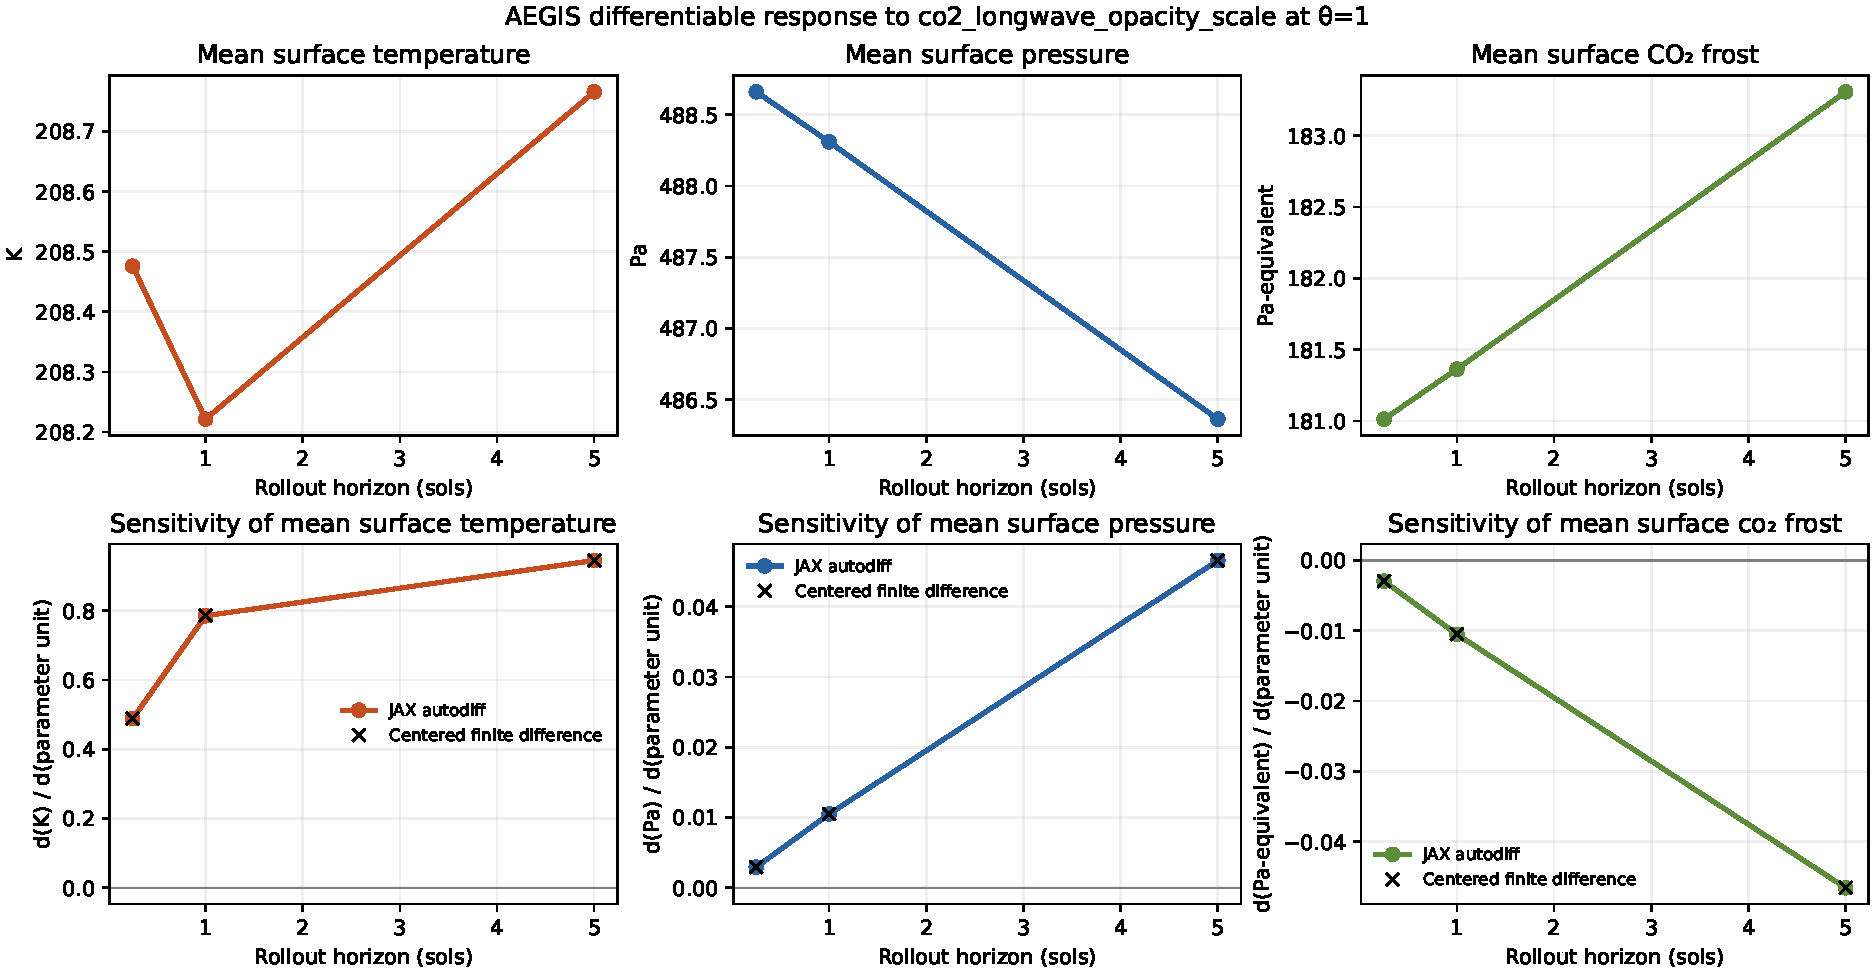
\includegraphics[width=0.85\linewidth]{co2-longwave-sensitivity.pdf}
\caption{Differentiable response of AEGIS to the \co{} longwave opacity multiplier $\beta$ at $\beta=1$, from a MY32, $L_s=45^\circ$ window. Top: global-mean surface temperature, surface pressure, and surface \co{} frost at rollout horizons of 0.25, 1, and 5 sols. Bottom: their derivatives with respect to $\beta$ computed by forward-mode automatic differentiation through the full coupled rollout (lines) and by centered finite differences (crosses). The pressure and frost sensitivities are equal and opposite, reflecting conservation of the atmosphere--frost \co{} inventory.}
\label{fig:co2-sensitivity}
\end{figure}

The historical twelve-window pilot reduces test temperature RMSE from 2.45505 to 2.39699\,K, a 0.05805\,K gain (Table~\ref{tab:skill}). A paired-year percentile interval conditional on the two held-out Mars years is [0.03512, 0.08693]\,K; four windows and one fitted run do not establish population skill or optimizer uncertainty. Training loss was still decreasing over the last five of the 50 Adam updates, so convergence was not established. The validation-selected physical controls were (0.902924, 1.096341, 0.816336). These historical results require regeneration after the PBL and sidereal-clock fixes; the revised runner records bounded multi-start optimizer termination and projected gradients rather than equating a fixed update budget with convergence.

\begin{table}[t]
\centering\small
\caption{Twelve-window reanalysis pilot: atmospheric temperature RMSE (K) at a single lead of 7397.937\,s. Each split contains four seasonally distributed windows, combined as the square root of their mean squared errors. The physical baseline is shared by the two fitting experiments.}
\label{tab:skill}
\begin{tabular}{lrrr}
\toprule
Configuration & Training & Validation & Test \\
\midrule
Physical baseline & 2.45 & 2.49 & 2.46 \\
Calibrated physics & 2.38 & 2.44 & 2.40 \\
Coupled neural heating & 2.42 & 2.49 & 2.46 \\
\bottomrule
\end{tabular}
\end{table}



\subsection{Computational performance and long integrations}
\label{sec:performance}

Published v1 reports an 86.6-minute one-year integration and an 11.4-hour ten-year integration at T21/L12, 450\,s, float64. These are historical reports, not newly reproduced timings: the original GPU is identified only as \texttt{cuda:0}, and a complete public release of the headline fields, spinup, and timing inputs is pending. We withdraw the relative speed claim against NASA Ames because hardware, physics, grid, and output costs were not matched. The reproducibility guide specifies synchronized forward/gradient timings and separates compilation, warmup, and execution.

The available annual ablation archive instead uses 300\,s, with a 150\,s paired trajectory. Reanalysis of their 74 common output times gives 3.700\,K equal-snapshot RMS temperature separation and 3.884\,K under trapezoidal time weighting. These are transient sensitivity statistics, not climatological error estimates or a 450/300\,s certification. Finite saved states do not establish physical realism or equilibration. Small post-projection inventory residuals must be reported separately from raw mass change and correction-induced energy and momentum changes. Differences between year-nine and year-ten global means must not be interchanged with spatial RMS differences; the headline metric definitions and raw fields remain to be reconciled.

\subsection{Seasonal comparisons with MOLA topography}
The MOLA-based lower boundary produces a strong geographic structure in surface pressure \citep{smith2001, mola}. Elevated regions contain less atmospheric column mass, while low-lying terrain supports higher surface pressure. Across our twelve season--reference comparisons, surface-pressure pattern correlations range from 0.975 to 0.989 (Table~\ref{tab:reference}). The model reproduces the terrain-driven hydrostatic pressure structure set by the MOLA lower boundary across all four seasons and all three reference products. Figure~\ref{fig:maps} shows the terrain context and the seasonal fields at $L_s=135^\circ$.

Surface-temperature correlations range from 0.732--0.821, but all twelve archived temperature biases are positive (+2.355 to +8.219\,K). Frost RMSE ranges from 123.036 to 631.330\,Pa-equivalent. Table~\ref{tab:reference} includes bias, RMSE, and correlation for all four fields, including frost and wind. High terrain-driven pressure correlation does not independently validate circulation or climatology.


The seasonal model uses opacity/exchange controls (0.25, 0.25, 1), selected after comparison with Ames; it is not an untuned or independent Ames validation. Calibration and neural baselines start at (1, 1, 1), while (0.6, 0.8, 1.4) is a synthetic teacher/gradient-test vector, not a fitted physical estimate. An independently calibrated, held-out seasonal evaluation remains required.

The seasonal comparison uses the documented sampling of each product: sparse model checkpoints within $\pm5^\circ$ of the target season, five-sol Ames averages, daily ARCO-MACDA averages, and four-local-time MCD means. Wind levels and frost averaging periods also differ between products. We interpret these as model and reanalysis comparisons.

\begin{figure}[!hbt]
\centering
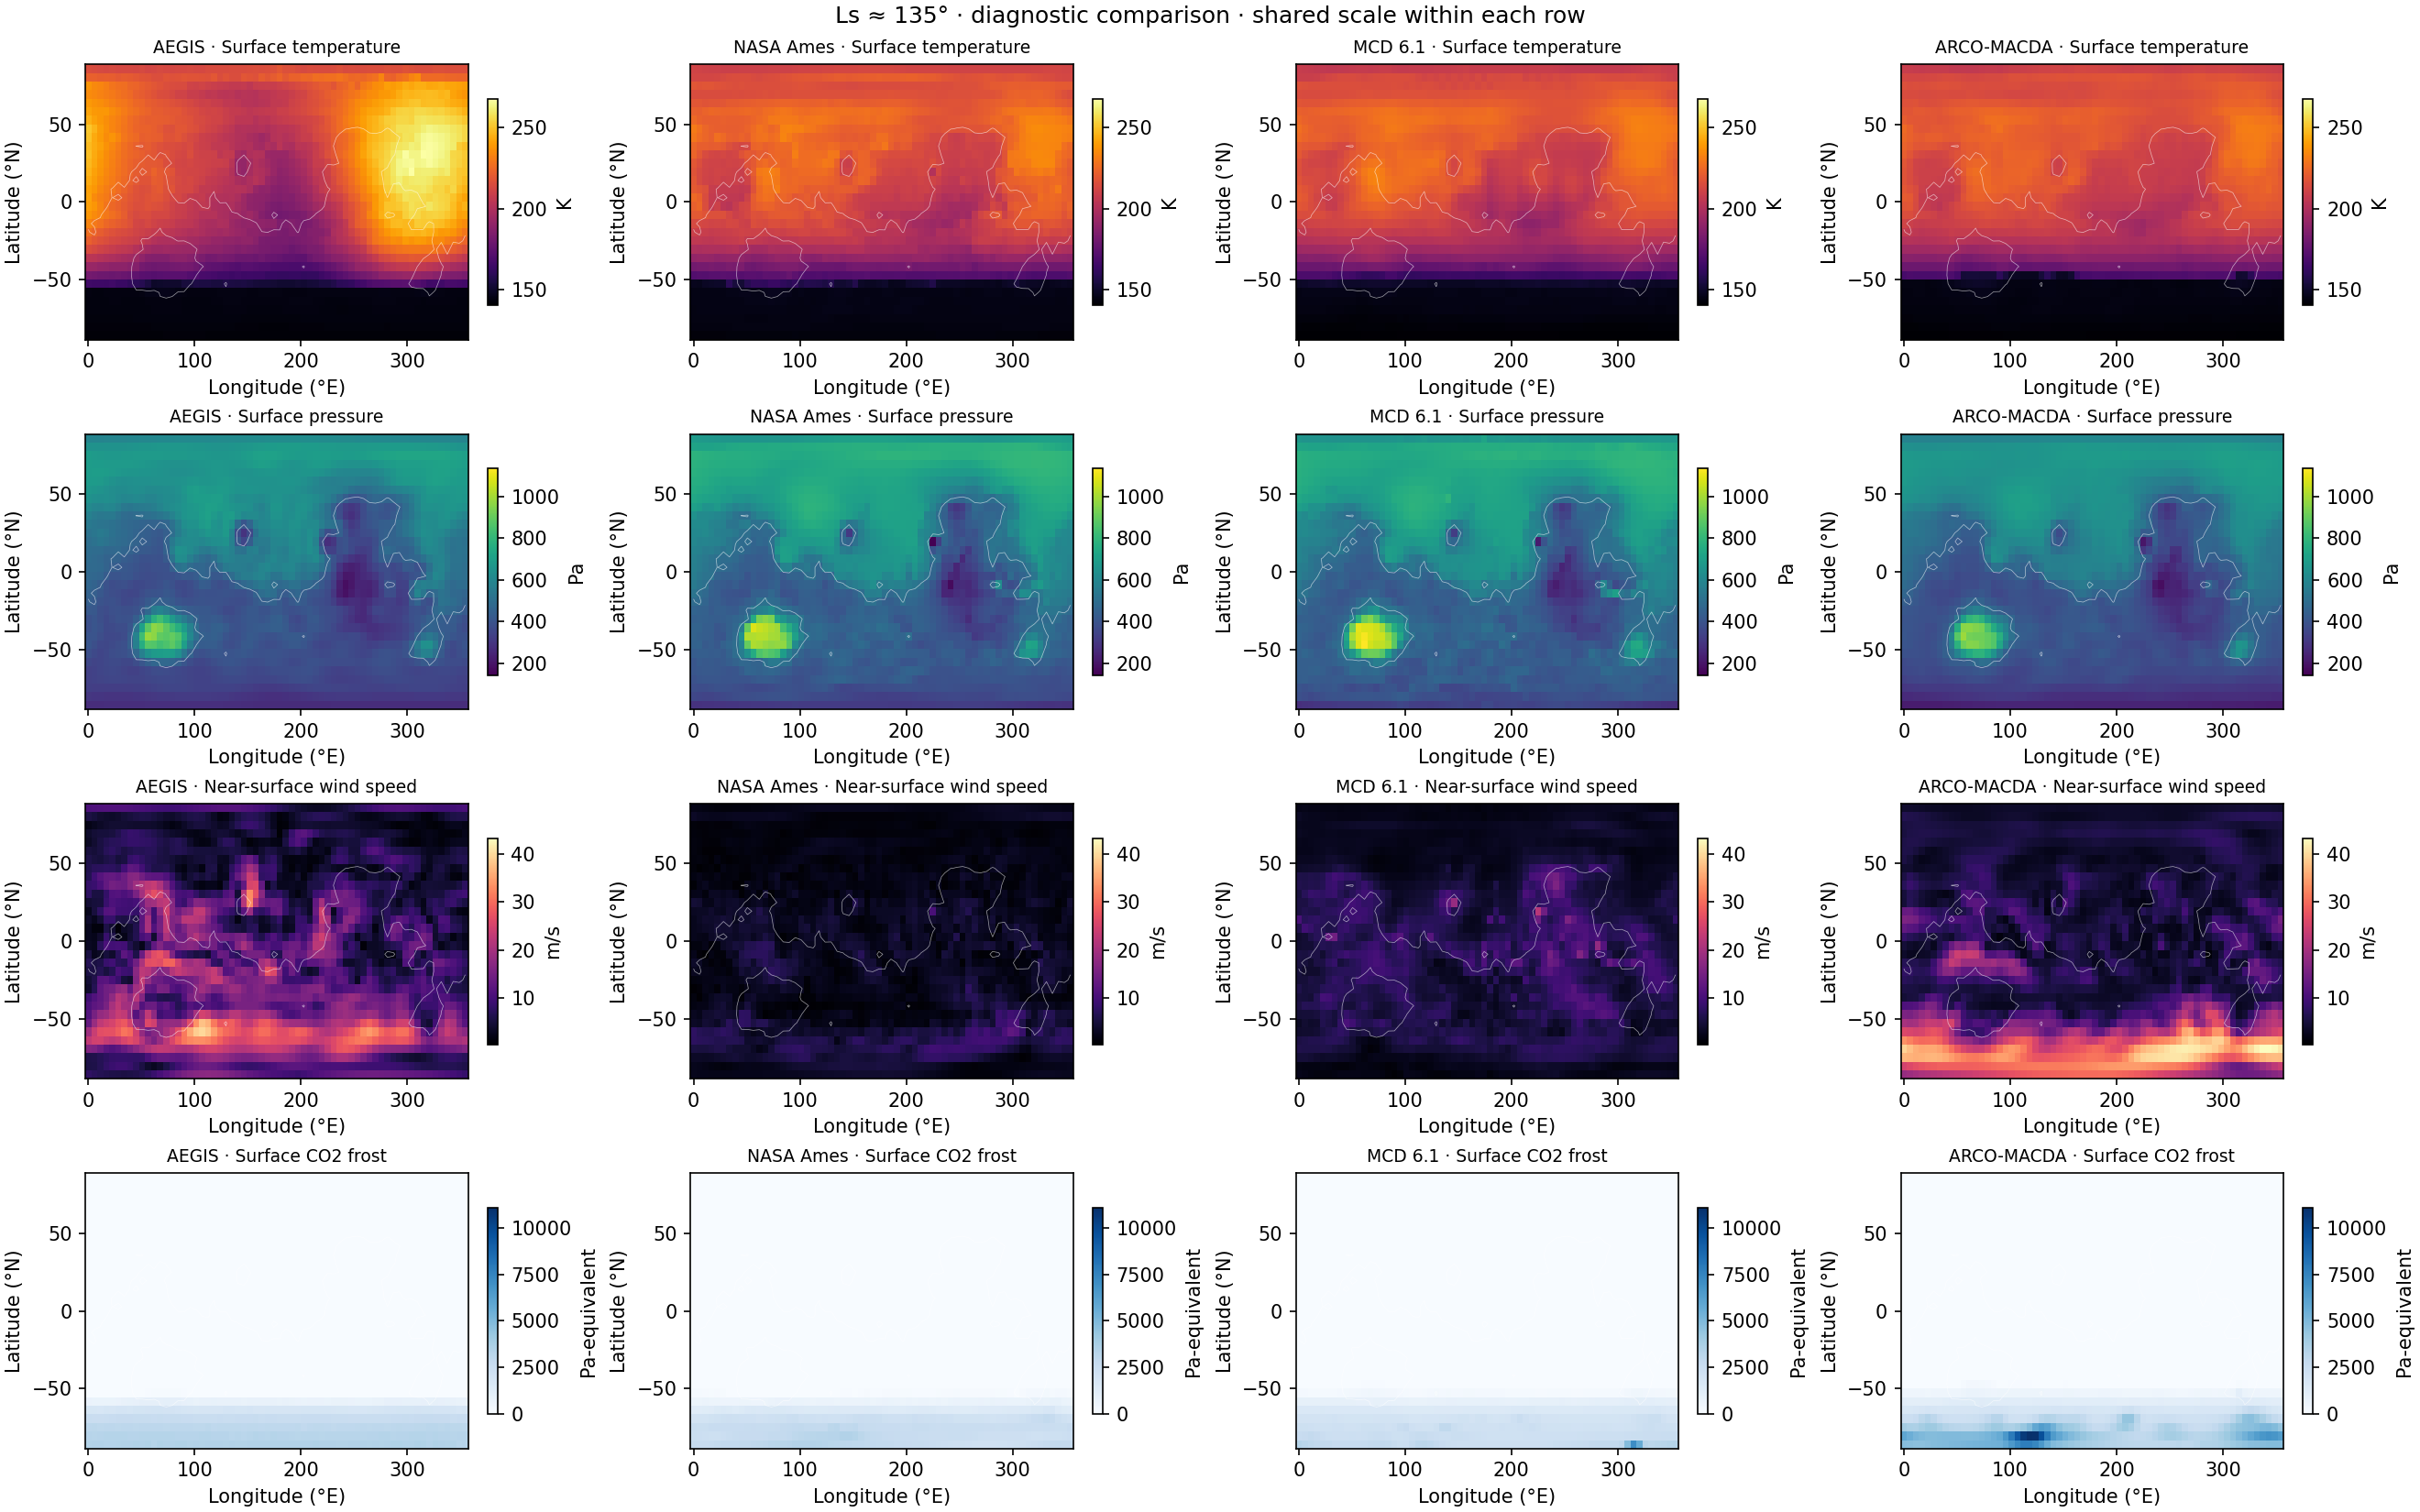
\includegraphics[width=\linewidth,height=.58\textheight,keepaspectratio]{ls135_grid.png}
\caption{MOLA terrain on the comparison grid (top), and seasonal fields at $L_s=135^\circ$ (bottom). The seasonal panels compare the physical model with NASA Ames, MCD 6.1, and ARCO-MACDA for surface temperature, pressure, near-surface wind speed, and surface \co{} frost.}
\label{fig:maps}
\end{figure}

% \subsection{Physical calibration against reanalysis}


% The selected physical multipliers are approximately 0.903 for \co{} longwave opacity, 1.096 for dust longwave opacity, and 0.816 for surface exchange. They are obtained by differentiating the coupled trajectory loss and updating all three controls together. The result demonstrates a practical use of differentiability: parameters are estimated against reanalysis while the atmosphere, radiation, and surface continue to interact during the forecast.

\begin{table}[t]\centering\small
\caption{Historical reference characterization, using the arithmetic mean of four seasonal statistics per row (not pooled spatial RMSE). Bias is model minus reference. Temporal sampling and wind heights are unmatched; opacity controls were Ames-informed.}
\label{tab:reference}\label{mola-table}
\begin{tabular}{llrrr}\toprule
Reference & Field & Bias & RMSE & Correlation \\\midrule
NASA Ames & Pressure (Pa) & -40.92 & 52.37 & 0.986 \\
NASA Ames & Temperature (K) & +3.46 & 20.64 & 0.789 \\
NASA Ames & Wind (m/s) & +9.75 & 11.91 & 0.442 \\
NASA Ames & Frost (Pa-eq.) & +7.31 & 168.48 & 0.816 \\
MCD 6.1 & Pressure (Pa) & -41.56 & 57.18 & 0.977 \\
MCD 6.1 & Temperature (K) & +7.12 & 21.58 & 0.787 \\
MCD 6.1 & Wind (m/s) & +6.91 & 10.03 & 0.263 \\
MCD 6.1 & Frost (Pa-eq.) & -5.69 & 196.28 & 0.806 \\
ARCO-MACDA & Pressure (Pa) & +3.43 & 40.72 & 0.988 \\
ARCO-MACDA & Temperature (K) & +7.42 & 22.27 & 0.772 \\
ARCO-MACDA & Wind (m/s) & +2.90 & 7.88 & 0.454 \\
ARCO-MACDA & Frost (Pa-eq.) & -65.55 & 368.34 & 0.795 \\
\bottomrule\end{tabular}\end{table}


\subsection{Physics ablations: process sensitivity}
We experiment with an ablation suite that pairs the full Mars configuration with twelve process perturbations, such as removing boundary-layer mixing, dry convection, regolith conduction, or \co{} exchange, \co{} longwave opacity, and dust longwave opacity. Each is launched from the same initial state, so any divergence traces to the changed process, and we report the root-mean-square (RMS) separation from the paired full-physics trajectory. At a 44\,400\,s horizon, the perturbations separate into a well-resolved sensitivity ranking (Fig.~\ref{fig:short-physics}): regolith conduction and boundary-layer mixing dominate, followed by dry convection and the surface-exchange multipliers, while the calibrated radiative opacity multipliers produce smaller but clearly resolved changes. Halving the time step changes temperature by only 0.0042\,K, a short-horizon numerical sensitivity check that does not certify long-horizon timestep convergence.

\begin{figure}[!hbt]
\centering
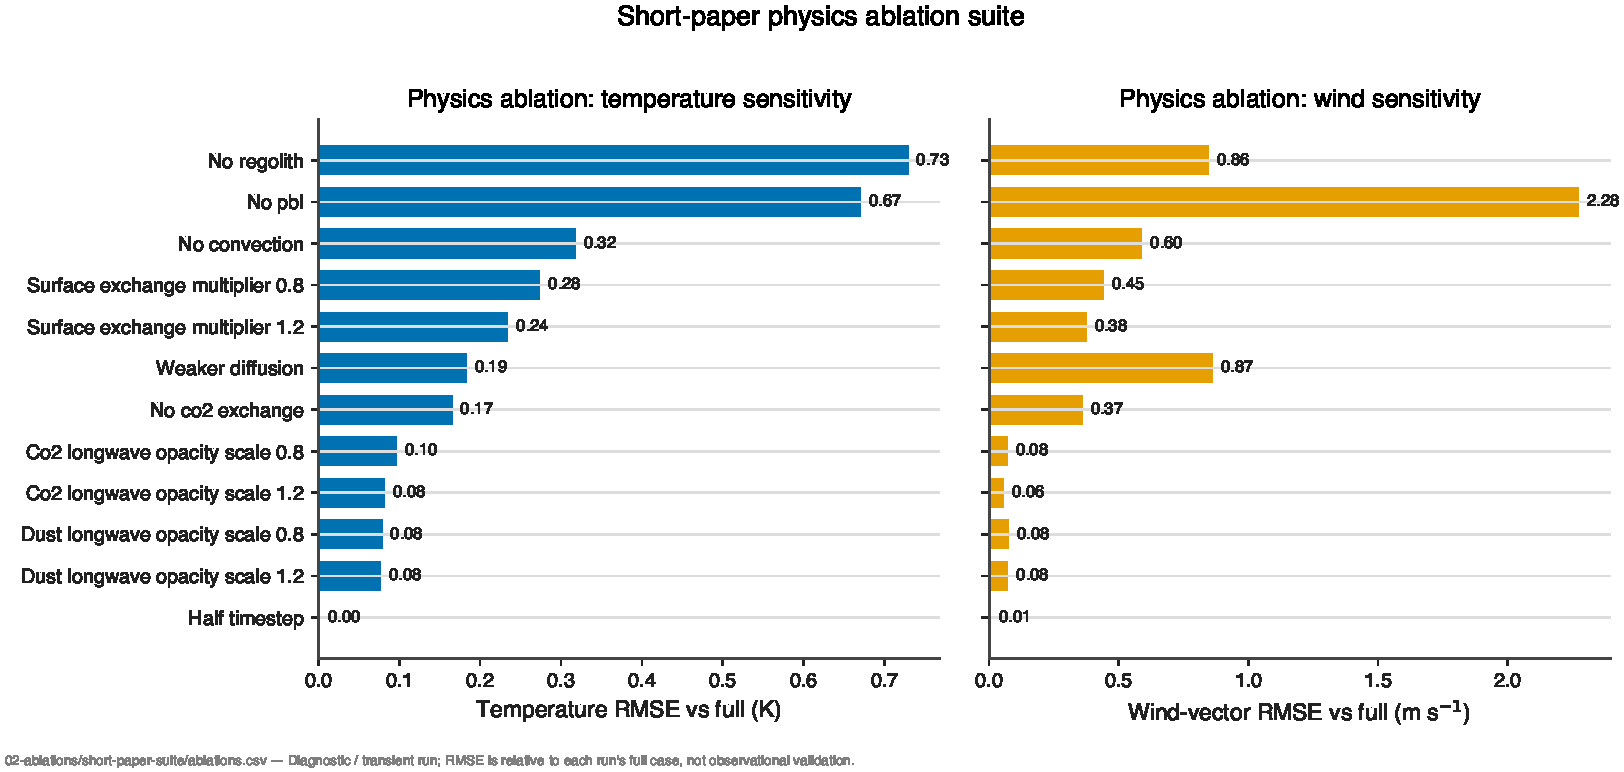
\includegraphics[width=0.9\linewidth]{short-ablations-rmse.pdf}
\caption{Sensitivity of the T21/L12 Mars configuration. Bars show RMS differences from the paired full-physics trajectory over five saved times through 44\,400\,s; the right panel combines zonal and meridional wind RMSE by quadrature. All cases begin from the same state.}
\label{fig:short-physics}
\end{figure}

% The ranking is corroborated on the year-long runs: at 88\,800\,s the half-step difference is still 0.0042\,K, against 1.169, 1.035, and 0.438\,K for regolith conduction, boundary-layer mixing, and \co{} exchange. 
% Extended to a full Mars orbital period (59\,356\,800\,s), 
All thirteen archived configurations complete with finite sampled states. The full-physics year's maximum relative post-projection inventory residual is $4.28\times10^{-9}$, which verifies the inventory constraint only. The same archive contains a peak wind of 236.046\,m\,s$^{-1}$, a minimum air temperature of 93.263\,K, and a sampled maximum Mach number of 1.098. Air reaches 35.77\,K below the model's layer-pressure \co{} frost point. These diagnostics motivate timestep, drag, and saturation studies rather than establishing a single cause or physical validity.




% can \subsection{Short-run physics sensitivity}
% In a paired 44\,400\,s experiment, the full Mars configuration and twelve perturbations start from the same state. Differences are measured against the full-physics trajectory at five saved times. Removing regolith conduction changes atmospheric temperature by 0.732\,K root mean square (RMS), and removing boundary-layer mixing changes it by 0.673\,K (Fig.~\ref{fig:short-physics}). The corresponding wind-vector differences are 0.855 and 2.283\,m\,s$^{-1}$. Halving the time step changes temperature by only 0.0042\,K over these samples. Throughout both sensitivity suites, RMS quantifies each process's coupled influence as the trajectory separation it produces from the paired full-physics run.

% \begin{figure}[!hbt]
% \centering
% 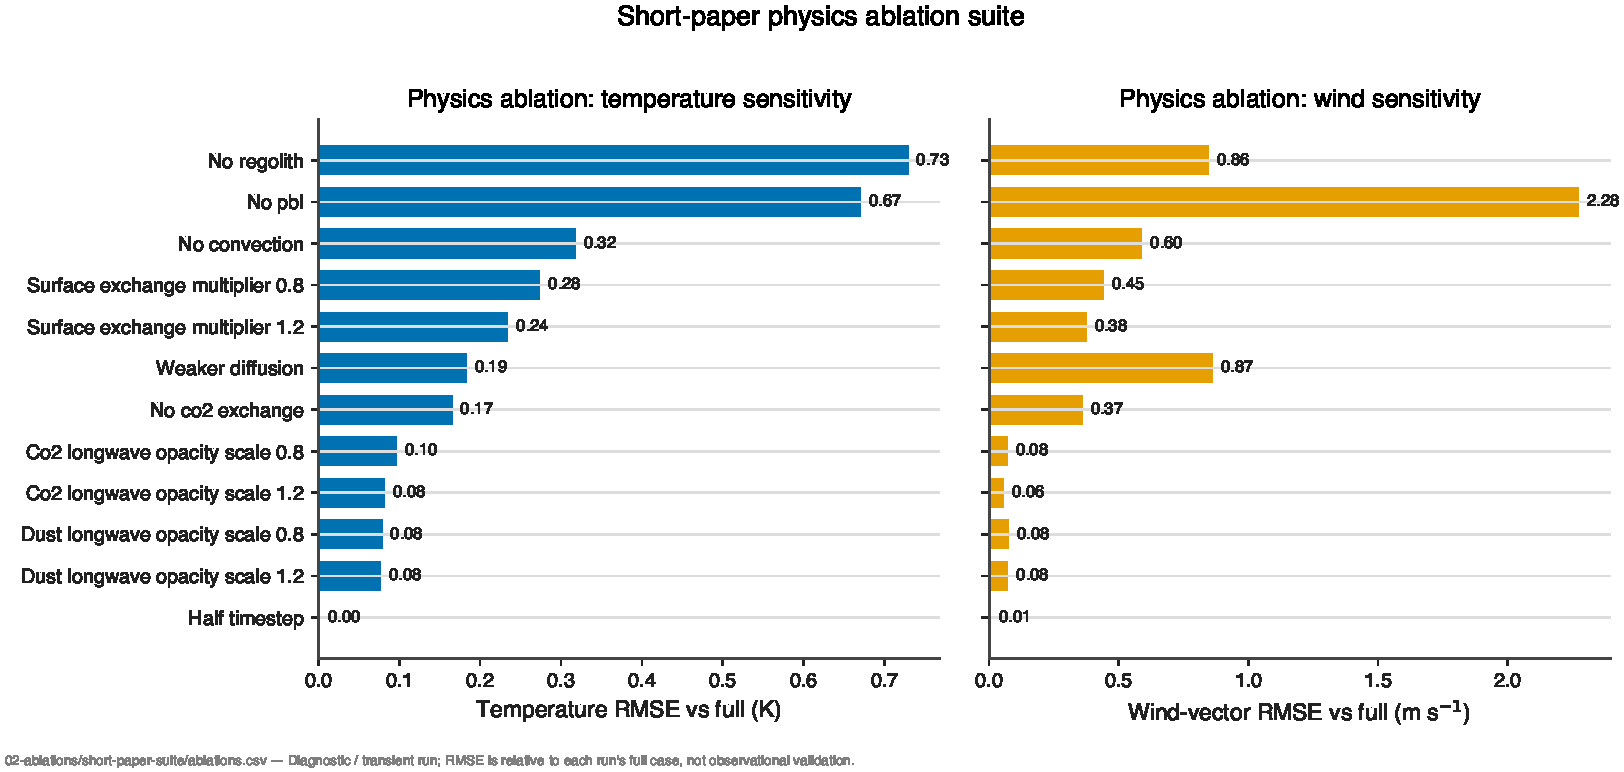
\includegraphics[width=\linewidth]{short-ablations-rmse.pdf}
% \caption{Short-run sensitivity of the T21/L12 Mars configuration. Bars show RMS differences from the paired full-physics trajectory over five saved times through 44\,400\,s; the right panel combines zonal and meridional wind RMSE by quadrature. All cases begin from the same state.}
% \label{fig:short-physics}
% \end{figure}

% \subsection{Annual integration and sensitivity}
% The annual suite evaluates a full-physics baseline and twelve perturbations over 59\,356\,800\,s, one adopted Mars orbital period. The perturbations remove boundary-layer diffusion, dry convection, regolith conduction, or \co{} exchange; weaken horizontal diffusion; halve the time step; or change one of the three physical multipliers by 20\%. Four computational partitions share the same initial restart and reproduce the same baseline. The merged result counts that baseline once.

% All thirteen configurations complete with finite sampled states. The largest temperature separation from full physics occurs when \co{} exchange is removed: 5.009\,K, with zonal- and meridional-wind differences of 10.522 and 9.902\,m\,s$^{-1}$ (Fig.~\ref{fig:annual}). Removing regolith conduction gives a temperature difference of 4.144\,K, followed by boundary-layer diffusion at 3.950\,K and dry convection at 3.792\,K. These runs show that the process switches affect the coupled solution.

% Each bar pools squared field differences over 74 saved times and 12 sigma layers using horizontal Gaussian area weights, then takes the square root. Saved times receive equal weight, including the more closely spaced samples near initialization.

% The 20\% parameter changes produce temperature differences of 3.531--3.867\,K. Halving the time step produces a difference of 3.700\,K over the annual sampling period, comparable to several physical perturbations. The saved early-time fields clarify this result. At 88\,800\,s, the half-step difference is only 0.0042\,K, compared with 1.035\,K after removing boundary-layer diffusion, 1.169\,K after removing regolith conduction, and 0.438\,K after removing \co{} exchange. By later times, freely evolving trajectories have separated substantially even under the smaller time step.

% The full-physics run has maximum relative total \co{} inventory drift of $4.28\times10^{-9}$. Every annual configuration remains below $8.55\times10^{-9}$ in this diagnostic. This verifies the operation of the atmosphere--frost inventory correction over long integrations while allowing seasonal exchange between reservoirs. The annual calculations are restart-based transients; the experiment tests numerical completion and sensitivity over a Mars year.


% \begin{figure}[t]
% \centering
% \includegraphics[width=\linewidth]{year-ablations.pdf}
% \caption{One-Mars-year trajectory sensitivity. Each bar is the root mean squared difference from the shared full-physics run, using area weights and equal weights across 12 layers and 74 saved times. The half-time-step case supplies numerical context. Four compatible partitions contribute twelve perturbations and one shared baseline.}
% \label{fig:annual}
% \end{figure}




% % \subsection{Computational cost of differentiable experiments}
% % The archived GPU timing experiment evaluates a T21/L12 trajectory to 22\,200\,s, sampled at 6000, 12\,000, and 22\,200\,s. The median of three synchronized warm evaluations is 2.125\,s for the forward trajectory and 8.719\,s for the loss with three forward tangents. These correspond to approximately 423.7 and 103.3 simulated sols per wall-clock hour for their respective workloads. The derivative workload costs about 4.10 times the forward evaluation in this experiment.

% % Recorded compilation times are 13.81 and 44.39\,s, respectively. Execution includes sampled field decoding and excludes input loading, compilation, and warmup. The measurements show that repeated gradient evaluations are practical once the workload hereis compiled. They also make the cost of derivative information explicit for designing calibration experiments. The archive identifies a single NVIDIA RTX A4000 GPU with float64 arithmetic.


\subsection{Neural components as coupled experiments}
AEGIS exposes learned components through the same operator interface as its physical parameterizations. A neural module attaches at a chosen process either as a bounded additive residual or as a full component replacement. Because the module enters the coupled step, its effect propagates through the subsequent dynamics and physics, and it is trained by differentiating the resulting trajectory. We showcase two experiments using these interfaces exposed by the framework.
% The coupled neural-heating experiment exercises the full path from current-state features to learned tendencies, time stepping, trajectory loss, and reverse-mode updates. Zero-output initialization reproduces the physical baseline within the recorded identity tolerance. All directional gradient checks pass. Over 50 updates, normalized training loss falls from about 0.0419 to 0.0417, and the selected validation loss is about 0.0416.

% Temperature training RMSE decreases from about 2.45 to 2.42\,K. On the four test windows, the coupled neural configuration matches the physical baseline to within 0.003\,K (both round to 2.46\,K; Table~\ref{tab:skill}), confirming that inserting a learned tendency preserves the calibrated physical solution while opening it to optimization. The normalized objective combines temperature and both wind components. This pilot establishes a complete, gradient-checked coupled-learning path---from state-dependent features through time stepping and a trajectory loss to reverse-mode updates---ready for richer neural hypotheses within Mars physics.



\subsubsection{Learning radiative fluxes}
We replace the compact physical radiation kernel with a structured learned flux operator that preserves the discrete radiative budget. Four-layer columns are first trained locally for 100 updates. Starting from that common fit, trajectory fine-tuning and local continuation each use 20 fixed updates (seed 0). This is an update-budget accuracy comparison, not equal computational cost. The v1 wall-time continuation happened to perform 234 updates, so its 0.416/0.979\,K values are historical machine-dependent results and are not retained as the primary accuracy comparison. The new CPU float64 run and an independent repeat archive reports, histories, checkpoints, generated predictions, executed source hashes, and the actual update counts.

\begin{table}[t]\centering\small
\caption{Fixed-update, seed-0, 48-step column air-temperature RMSE (K). Both continuations start from the same 100-update local fit. Generated physical-kernel targets; not observational Mars skill.}
\label{tab:radiation_results}\begin{tabular}{lrr}\toprule
Training & Interpolation & Higher dust \\\midrule
Initial local fit & 0.620 & 1.799 \\
Trajectory, 20 updates & 0.566 & 1.653 \\
Continued local, 20 updates & 0.592 & 1.595 \\
\bottomrule\end{tabular}\end{table}


With fixed update counts, trajectory fine-tuning gives the lowest interpolation error (0.566\,K), while continued local fitting gives the lowest higher-dust error (1.595\,K). The local-fit baseline is 0.620/1.799\,K, and continued local fitting is 0.592/1.595\,K. Neither method wins on both splits. All variants complete the two-step T21 coupled execution check. The maximum held-out instantaneous radiation closure residual is $1.42\times10^{-14}$\,W\,m$^{-2}$; this component identity is not a full-GCM energy-conservation result. A repeated seed-0 run agrees within the recorded tolerance.


% Together with the heating experiment, this result demonstrates two supported
% learning interfaces: additive residual learning and replacement of a physical
% operator. 

\begin{figure}[!hbt]
\centering
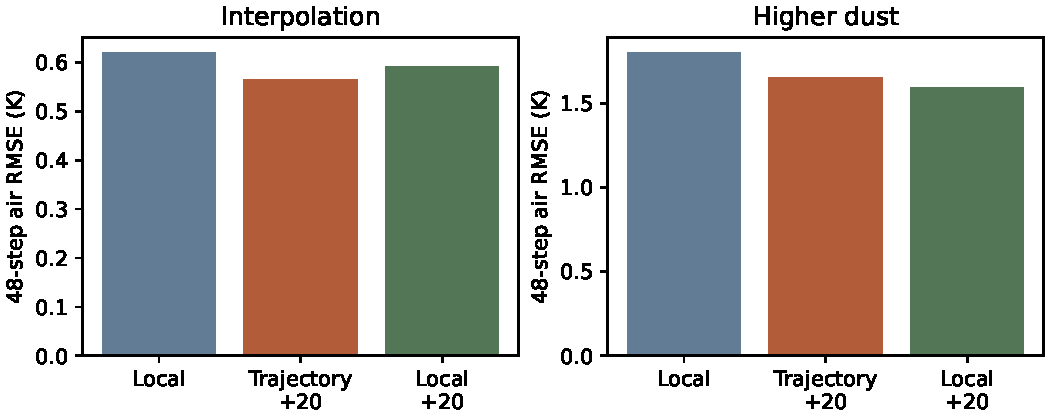
\includegraphics[width=0.85\linewidth]{neural-radiation-48step.pdf}
\caption{Fixed-update neural-radiation experiment at a 48-step column rollout (100 initial updates; 20 updates per continuation method; seed 0). Air-temperature RMSE is evaluated against the compact physical radiation kernel on held-out interpolation columns and higher-dust extrapolation columns (24 columns per split). The three bars compare the initial local fit, trajectory fine-tuning, and continued local fitting.}
\label{fig:neural-radiation}
\end{figure}

% \subsubsection{Optimizing a neural atmospheric control}
% A second experiment optimizes a bounded neural heating policy through the coupled model. The target is the final physical temperature field shifted by $-1.5$\,K. The archived run uses T21 with two layers, three 30\,s steps, and twelve optimization updates. The policy is constrained to heating magnitudes below $2\times10^{-4}$\,K\,s$^{-1}$, a strict physical bound that the optimizer respects exactly throughout training. Its final-state objective, including parameter regularization, decreases by 1.5\%, from 2.245 to 2.211, and the rollout remains finite. This experiment demonstrates end-to-end gradient-based optimization of a bounded, state-dependent heating policy through the coupled Mars model, using the same tendency interface as the neural closures.

\subsubsection{Recovering a physical parameter through a trajectory}
The differentiable column system recovers a known \(1.6\) multiplier on a bulk sensible-heat conductance of \(2\,\mathrm{W\,m^{-2}\,K^{-1}}\), using targets generated with fixed illumination, dust, and pressure per column. After 120 updates through 24-step trajectories, initial multipliers of
\(0.5\), \(1.0\), and \(3.0\) converge to \(1.59950\), \(1.59901\), and \(1.59696\), all within \(0.20\%\) of the target
(Fig.~\ref{fig:parameter-recovery}). Derivative checks at multipliers
\(0.5\), \(1.0\), and \(2.5\) agree with finite differences to relative discrepancies below \(3.41\times10^{-10}\). A derivative-free scalar reference reaches \(1.60000007\) in nine objective evaluations. This controlled recovery establishes parameter identifiability and a gradient-based inverse workflow through the shared differentiable column
operators.

\begin{figure}[!hbt]
\centering
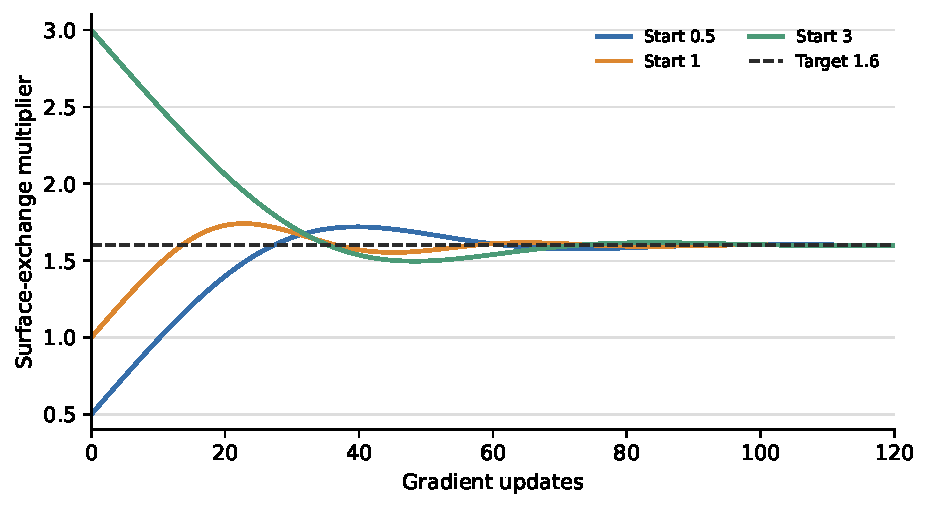
\includegraphics[width=.75\linewidth]{parameter-recovery.pdf}
\caption{Physical inverse experiment from the neural-framework archive. Gradient-based optimization recovers a prescribed surface-exchange multiplier of 1.6 from three initial values over 120 updates. Each curve includes its initial value and the saved multiplier after every update. The parameter belongs to the controlled column model; the experiment tests the shared differentiable inference workflow.}
\label{fig:parameter-recovery}
\end{figure}

\section{Future extensions}
% AEGIS connects a physically interpretable planetary model to the tools needed for differentiable experimentation. The same model supports forward climate integration, gradients with respect to physical parameters, and neural training through time. The Mars-specific work is concentrated in the operators that matter for its atmosphere: \co{} and dust radiation, surface and regolith energy storage, vertical exchange, and a condensable mass budget. This organization makes it possible to change one component while retaining the rest of the coupled system. The experiments also suggest a productive order for model development. Reference comparisons identify the spatial and seasonal fields to target. Physical calibration tests whether a small set of interpretable controls can reduce errors. Neural residuals or component r eplacements then provide additional hypotheses whose effects can be assessed with the same trajectory objectives and held-out windows.

% \paragraph{Scope and extension toward terraforming.}
The present demonstrations span coarse-resolution physical simulations, coupled-heating seed, and structured neural component replacement, and they establish the differentiable physical and neural interfaces. The framework already supports the natural next steps: broader observational comparison, repeated neural experiments across seeds, and multi-year equilibration studies, each reusing the same coupled operators and trajectory objectives. The explicit planetary, radiation, and reservoir interfaces provide a route to experiments with changing Martian boundary conditions. Altered surface albedo, imposed heating, or specified changes in volatile inventory could be introduced through these interfaces and evaluated    with spatial climate diagnostics. Differentiable objectives could then connect intervention parameters to quantities such as regional temperature, frost persistence, or atmospheric pressure. For larger changes in atmospheric composition and mass, the body thermodynamics, opacity data, condensable processes, and applicable dynamical assumptions would be extended together. 


\section{Conclusion}
AEGIS connects modular Mars operators to the Dinosaur dynamical core and differentiable physical and neural experiments. Archived gradient checks and controlled inverse experiments demonstrate useful discrete sensitivities. Historical reference comparisons expose temperature, wind, and frost errors and documented tuning; they do not establish independently validated climatology. The new fixed-update radiation comparison makes the learning budget reproducible and separates accuracy from machine-dependent timing. Converged reanalysis fitting, corrected-model seasonal and timestep studies, complete raw budget diagnostics, and a public release of the headline long-run fields remain necessary before stronger climate or performance claims.

\section*{Scope and reproducibility}
The \co{} cycle is surface-only: atmospheric condensation, latent heating aloft, and condensate sedimentation are absent. The frost relation uses the fixed-CO2/total-pressure approximation and is not a general gas-mixture calculation. Prescribed dust, equally spaced sigma levels, missing subgrid orographic drag, and numerical mass repairs limit long-run interpretation. A temperature clamp would not supply conservative missing physics. The revised implementation separates sidereal rotation (88642.663\,s) from the solar sol (88775.244\,s); historical nondimensional restarts must be reconstructed from dimensional fields before use with changed unit scales. Results from before and after these fixes must not be silently combined.

The repository archives the immutable arXiv v1 source, this revision, a claim-to-evidence map, the corrected radiation runs, and the recovered small-data calibration evidence under \texttt{paper/arxiv-2610.04081}. The simple command sequence in \texttt{docs/paper-reproduction.md} distinguishes executable small-data audits, fresh model runs, external inputs, and pending public fields. Historical figures retain their source revisions; only the fixed-update radiation figure is replaced by the new run. The revision does not assert that absent headline artifacts or new annual simulations have been reproduced.

% \section*{Code and data availability}
% The model repository contains the manuscript, local figure assets, machine-readable result tables, and experiment provenance. Figure locations and checksums are recorded in \texttt{figure-manifest.json}; derivative and fitting metrics are preserved in \texttt{evidence}. The accompanying script regenerates numerical tables and verifies headline metrics. External inputs include MOLA, TES-derived boundary fields, NASA Ames output, MCD 6.1, and ARCO-MACDA.

% \newpage

% \subsection*{AI use statement}
% We used generative AI tools in the following ways and have reviewed all AI-assisted work. We take responsibility for the final content of this work, including text, claims, and artifacts produced with the aid of generative AI.
% \begin{itemize}[leftmargin=*,nosep]
% \item \textbf{To aid or polish writing.} AI tools helped draft, condense, and reword manuscript text, including section summaries, captions, and the abstract and conclusion. All AI-assisted text was checked by the authors against the reported results, and every number in the paper was traced to its archived result file.
% \item \textbf{For retrieval and discovery.} AI tools helped identify related work and check bibliography entries against their Crossref, DataCite, and arXiv records. Every citation was verified against its DOI or arXiv record, and incorrect entries were corrected or removed.
% \item \textbf{For research ideation or execution.} AI tools suggested candidate experiments and helped write and test analysis, plotting, and auxiliary experiment scripts. The core model was written by the authors. AI-written scripts were inspected, tested with smoke and gradient checks, and run by the authors. No simulation outputs or numerical results were produced or altered by AI tools; all reported values come from executed model runs archived with the code.
% \end{itemize}

% \subsection*{Ethics statement}

% (This section is \textbf{recommended} and does not count toward the page limit.)

% If authors feel that their paper submission raises questions regarding the Code
% of Ethics, they are encouraged to include a paragraph of Ethics Statement (at
% the end of the main text before references) to address potential concerns where
% appropriate. Topics include, but are not limited to, studies that involve human
% subjects, practices to data set releases, potentially harmful insights,
% methodologies and applications, potential conflicts of interest and sponsorship,
% discrimination/bias/fairness concerns, privacy and security issues, legal
% compliance, and research integrity issues (e.g., IRB, documentation, research
% ethics). This statement should not be more than 1 page.

% \subsection*{Reproducibility statement}

% (This section is \textbf{recommended} and does not count toward the page limit.)

% It is important that the work published in ICLR is reproducible. Authors are
% strongly encouraged to include a paragraph-long Reproducibility Statement at the
% end of the main text (before references) to discuss the efforts that have been
% made to ensure reproducibility. This paragraph should not itself describe
% details needed for reproducing the results, but rather reference the parts of
% the main paper, appendix, and supplemental materials that will help with
% reproducibility. For example, for novel models or algorithms, a link to an
% anonymous downloadable source code can be submitted as supplementary materials;
% for theoretical results, clear explanations of any assumptions and a complete
% proof of the claims can be included in the appendix; for any datasets used in
% the experiments, a complete description of the data processing steps can be
% provided in the supplementary materials. Each of the above are examples of
% things that can be referenced in the reproducibility statement.

% \subsubsection*{Author Contributions}
% If you'd like to, you may include  a section for author contributions as is done
% % in many journals. This is optional and at the discretion of the authors.

% \subsubsection*{Acknowledgments}
% Use unnumbered third level headings for the acknowledgments. All
% acknowledgments, including those to funding agencies, go at the end of the paper.


\bibliography{iclr2027_conference}
\bibliographystyle{iclr2027_conference}

\appendix
\section{Mars physics operators}\label{app:physics}

MOLA elevation data provide the lower boundary \citep{smith2001,mola}. The raster is regridded onto the transform grid and converted into spectral orography. Prescribed dust fields can be supplied through seasonal or per-window adapters. These data remain separate from the numerical operators, making boundary-condition experiments straightforward.

Radiation combines \co{} absorption and dust optical properties in a column flux calculation. The correlated-$k$ approach represents nongray gaseous absorption using a reduced distribution of absorption coefficients \citep{lacis1991}. The main physical configuration uses bundled Ames-derived 12-band correlated-$k$ tables, interpolated in temperature and log pressure, together with two-stream transfer. Solar and thermal fluxes are evaluated at layer interfaces, and atmospheric heating follows from their convergence. For layer $k$, with pressure thickness $\Delta p_k=p_s\Delta\sigma_k$, the atmospheric heat capacity per unit area is
\begin{equation}
 C_k=\frac{c_p\Delta p_k}{g},\qquad
 \left.\frac{dT_k}{dt}\right|_{\mathrm{rad}}=\frac{Q_k}{C_k},
\end{equation}
where $Q_k$ is radiative flux convergence. Computing atmospheric and surface heating from a common set of interface fluxes makes the column energy exchanges telescope to the top-of-atmosphere balance. This same construction is used for the neural radiation interface.

The surface temperature evolves from radiative, sensible, conductive, and latent heat exchange \citep{forget1999,haberle2019ames}. A bulk aerodynamic sensible heat flux couples the surface to the lowest atmospheric layer. The surface loss and atmospheric gain use the same flux, with atmospheric heating divided by the layer heat capacity. Surface stress transfers momentum, and Richardson-number-dependent vertical diffusion mixes momentum, heat, and tracers. The boundary-layer physics is motivated by \citet{petrosyan2011pbl}; the implementation uses a batched tridiagonal linear solve. Dissipated resolved kinetic energy is returned as heat. Dry convective adjustment mixes unstable adjacent layers while conserving their sigma-weighted enthalpy. A 12-layer regolith conducts heat beneath the surface and supplies thermal memory across daily and seasonal forcing.

The \co{} cycle couples temperature to atmospheric mass. Surface condensation releases latent heat and transfers mass from the atmosphere to frost; sublimation reverses the exchange. The local phase-change contributions satisfy
\begin{equation}
 \left.\frac{dp_s}{dt}\right|_{\mathrm{phase}}=-\frac{dI}{dt},
 \qquad
 \left.\frac{d\log p_s}{dt}\right|_{\mathrm{phase}}
 =-\frac{1}{p_s}\frac{dI}{dt}.
\end{equation}
The frost temperature follows a pressure-dependent saturation relation, and an energy-limited option ties the exchange to the surface energy budget. After each complete time step, a projection repairs negative frost and transfers the corresponding deficit from the atmospheric column. A global pressure rescaling then matches the quadrature-integrated atmosphere-plus-frost inventory to its pre-step value, accounting for prescribed escape when enabled. This addresses the finite-step inventory error associated with advancing log pressure. Atmospheric pressure can still change seasonally as mass moves into and out of the surface reservoir.


\section{Calibration and neural-training protocol}\label{app:protocol}

Physical calibration and coupled heating are evaluated using twelve prespecified ARCO-MACDA reanalysis windows \citep{arcomacda,macda}. Four windows from Mars years 24, 26, 29, and 31 are used for training; four from years 32--33 for validation; and four from years 34--35 for testing. Each split samples four seasonal quarters. Atmospheric initial conditions are constructed from the reference temperature, winds, and pressure. Surface and frost initialization use start-time fields, and the soil initialization uses preceding surface history. The native reference interval of 7397.937\,s is integrated with 25 steps of 295.91748\,s. Start-time dust and the orbital phase are matched for each window.

The training loss averages squared errors in temperature, zonal wind, and meridional wind, after scaling each field by its training-target standard deviation. It uses horizontal area weights, equal sigma-layer weights, and equal window weights. Feature normalization uses initial states from training data. Both fitting experiments perform 50 Adam updates \citep{kingma2014} with learning rate $10^{-3}$ and gradient-norm clipping at one. Validation selects the checkpoint, including the initial physical baseline among the candidates. Physical calibration adjusts \co{} longwave opacity, dust longwave opacity, and surface exchange within bounds $[0.05,2]$, $[0.05,2]$, and $[0.25,4]$. Neural fitting retains all three physical multipliers at one. Reported split RMSE is the square root of the mean per-window MSE, matching the figure-generation code.

\section{Additional seasonal reference comparisons}\label{app:seasonal-maps}
Figure~\ref{fig:maps} in the main text shows the seasonal fields at $L_s=135^\circ$. Figures~\ref{fig:maps-ls045} and~\ref{fig:maps-ls315} give the remaining aphelion-side and perihelion-side seasons, $L_s=45^\circ$ and $L_s=315^\circ$, under the same sampling conventions and the same set of reference products. The Ls225 transition-season panel is also included below; the table covers all four seasons and retains the historical sampling qualifications.

\begin{figure}[!hbt]
\centering
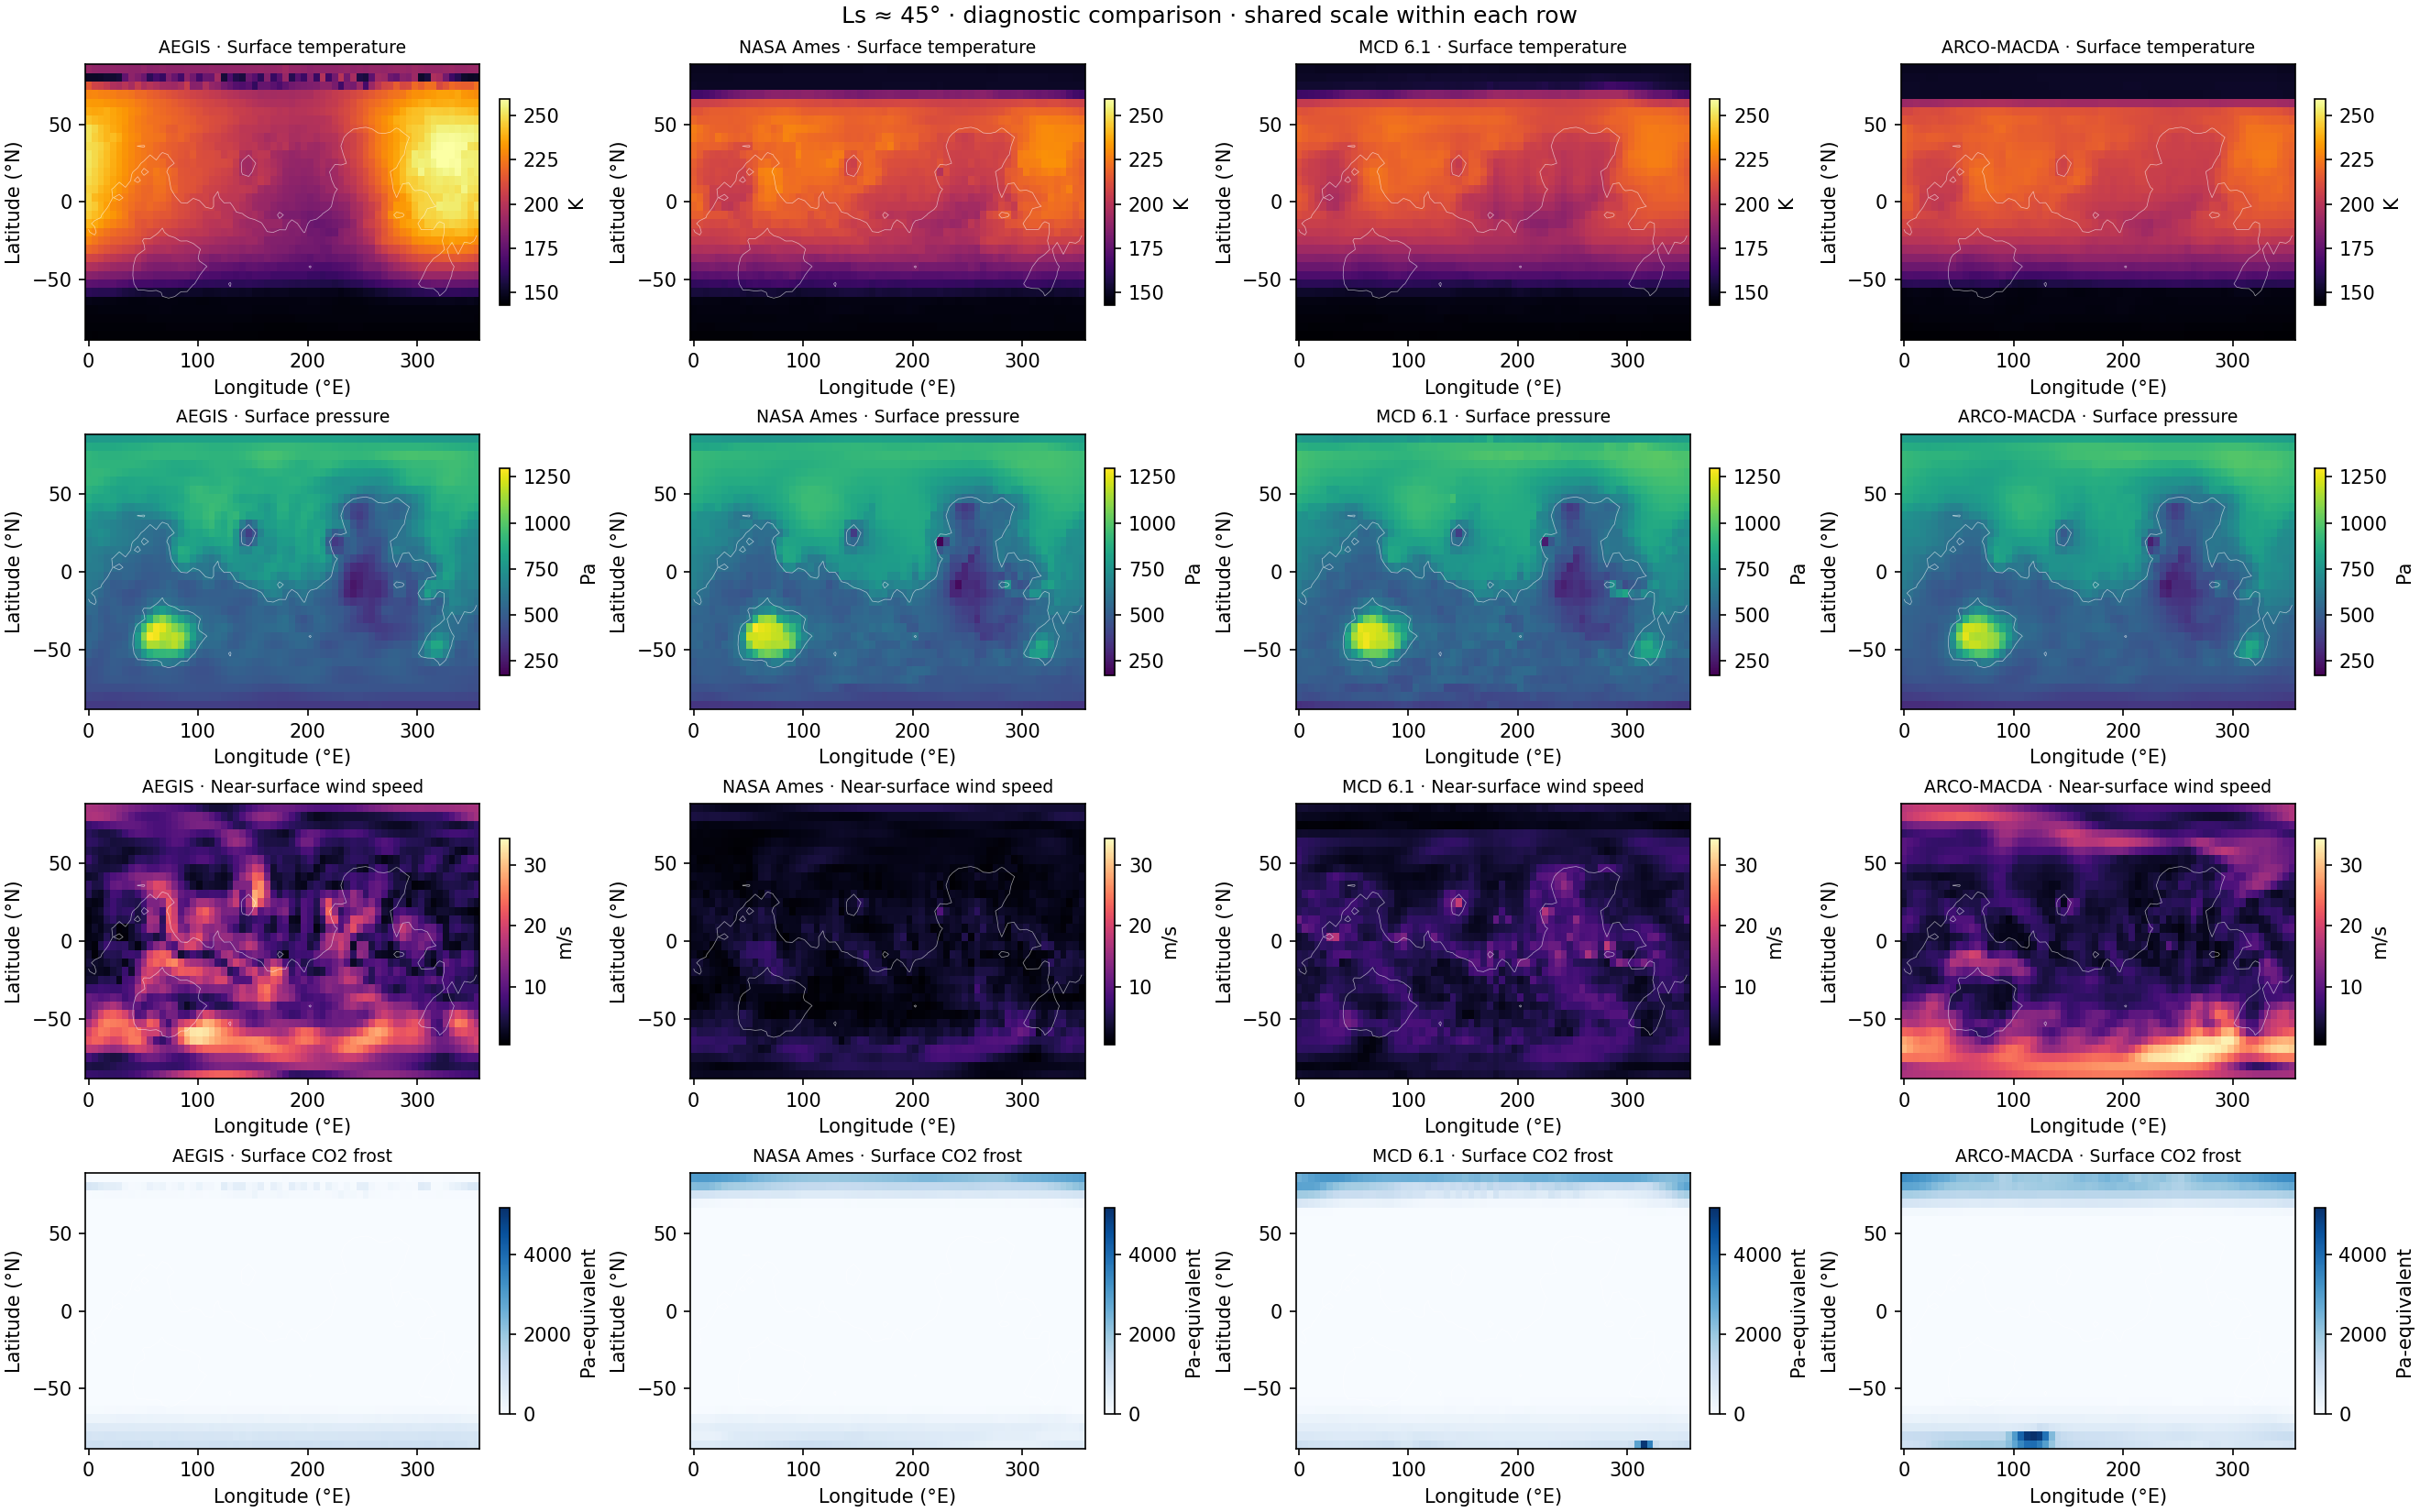
\includegraphics[width=\linewidth,height=.58\textheight,keepaspectratio]{ls045_grid.png}
\caption{Seasonal fields at $L_s=45^\circ$. The panels compare the physical model with NASA Ames, MCD 6.1, and ARCO-MACDA for surface temperature, pressure, near-surface wind speed, and surface \co{} frost, under the sampling conventions described in the main text.}
\label{fig:maps-ls045}
\end{figure}

\begin{figure}[!hbt]
\centering
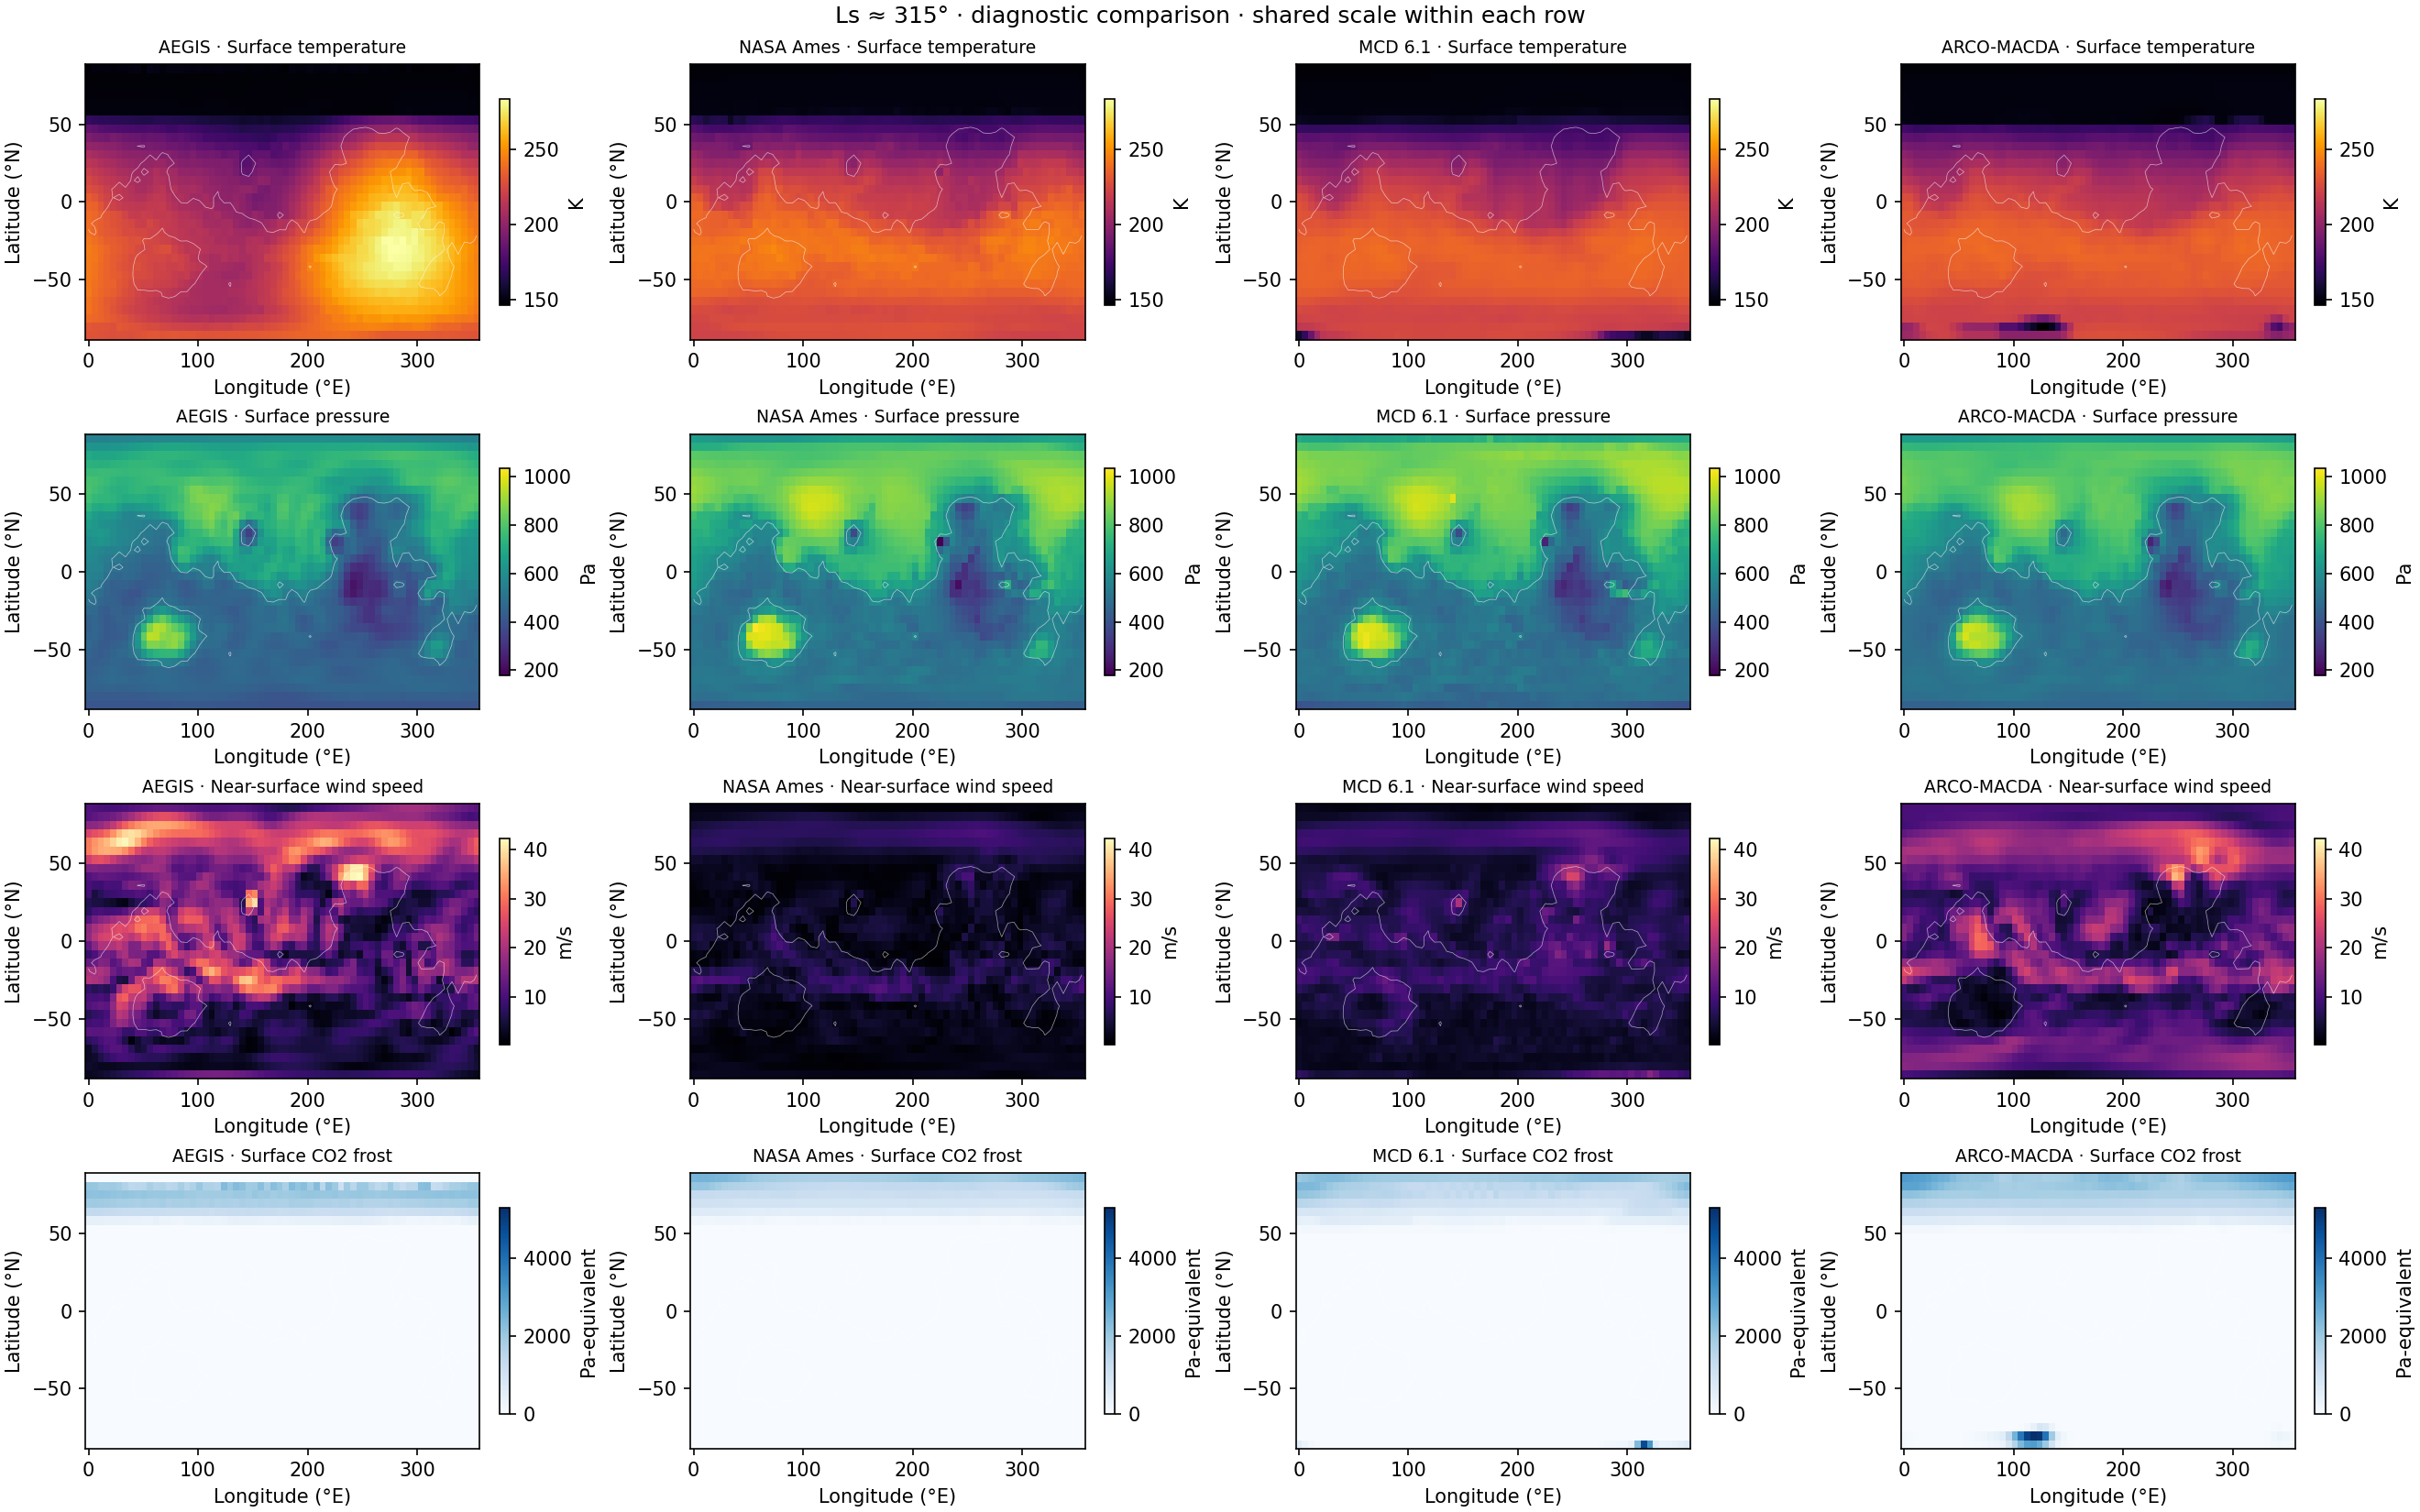
\includegraphics[width=\linewidth,height=.58\textheight,keepaspectratio]{ls315_grid.png}
\caption{Seasonal fields at $L_s=315^\circ$. The panels compare the physical model with NASA Ames, MCD 6.1, and ARCO-MACDA for surface temperature, pressure, near-surface wind speed, and surface \co{} frost, under the sampling conventions described in the main text.}
\label{fig:maps-ls315}
\end{figure}

\begin{figure}[!hbt]
\centering
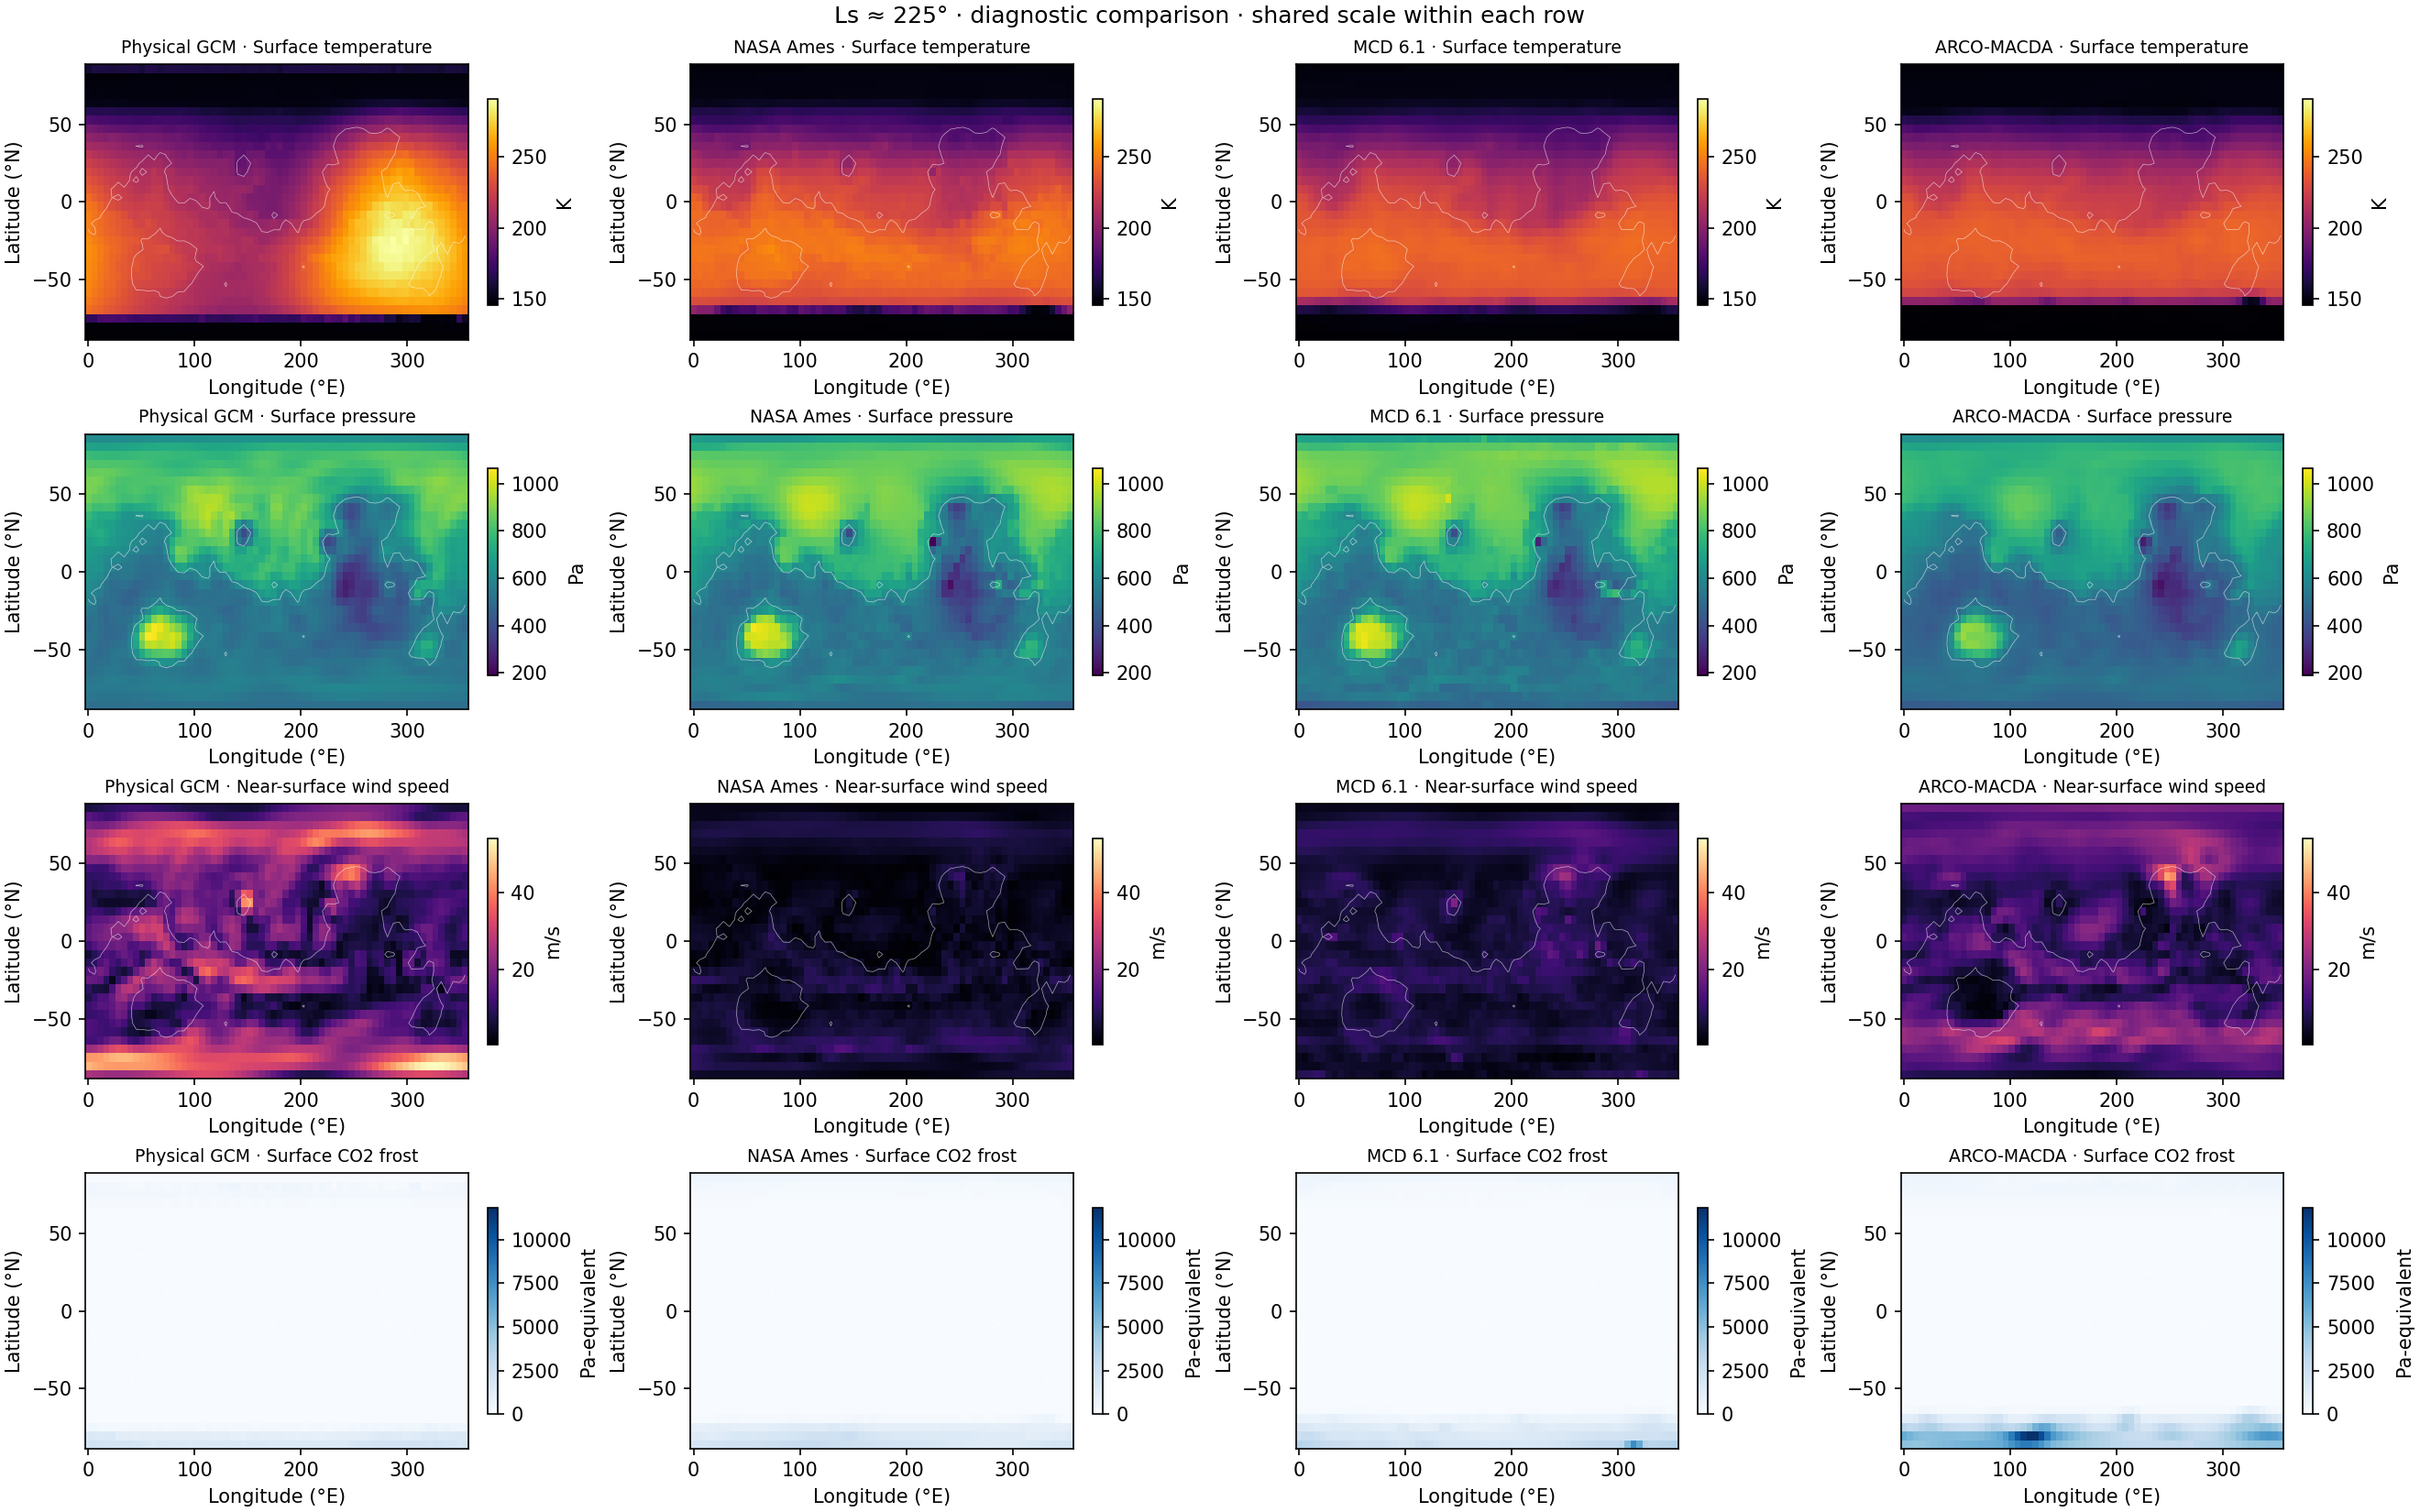
\includegraphics[width=\linewidth,height=.58\textheight,keepaspectratio]{ls225_grid.png}
\caption{Seasonal diagnostic comparison at $L_s=225^\circ$, organized as a $4\times4$ grid. Each \emph{row} is one surface field---surface temperature (K), surface pressure (Pa), near-surface wind speed (m\,s$^{-1}$), and surface \co{} frost (Pa-equivalent)---and each \emph{column} is one source: the AEGIS physical model (leftmost) alongside the NASA Ames, MCD~6.1, and ARCO-MACDA reference products. All panels are longitude--latitude maps ($0$--$360^\circ$E, $90^\circ$S--$90^\circ$N) with the MOLA terrain contour overlaid for geographic reference, and the color scale is shared within each row so the model and the three references are directly comparable field by field. Reading across a row shows how closely the modeled field tracks each reference; reading down the leftmost column shows the modeled state across all four diagnostics. Table~\ref{tab:reference} summarizes the corresponding pattern correlations and RMSE.}
\label{fig:maps-ls225-grid}
\end{figure}

\end{document}
